
\newcommand{\npattern}{31}
\newcommand{\ngroup}{10}
\newcommand{\nprim}{250}
\newcommand{\nbrokenlinks}{221}


\newcommand{\castpatternsection}[1]{\noindent\textbf{#1.}}
\newcommand{\pname}[1]{\textsc{#1}}
\newcommand{\group}[1]{

\

\

{\noindent\Large Patterns for \textsc{#1}}

\

% \begin{figure}[ht!]
% \centering
% \includegraphics[width=\textwidth]{"analysis/table-patterns-5000-by-group-#1"}
% \caption{#1 Cast Pattern Occurrences}
% \label{fig:group-patterns:#1}
% \end{figure}

}


\newenvironment{pattern}[1]{
\newcommand{\nocc}{\csname n#1Pattern\endcsname{}}
\newcommand{\noccsrc}{\csname n#1PatternSrc\endcsname{}}
\newcommand{\noccgen}{\csname n#1PatternGen\endcsname{}}
\newcommand{\nocctest}{\csname n#1PatternTest\endcsname{}}
\newcommand{\pocc}{\csname p#1Pattern\endcsname{}}

\newcommand{\desc}{\castpatternsection{Description}}
\newcommand{\instances}{\castpatternsection{Instances: \nocc{} (\pocc\%)}
We found \noccsrc{} in application code, \nocctest{} in test code, and \noccgen{} in generated code.}
\newcommand{\discussion}{\castpatternsection{Discussion}}
\newcommand{\thisp}{\textsc{#1}}
\subsection{\pname{#1}}
\label{pat:#1}
\desc
}{}


\section{Cast Usage Patterns}
\label{sec:casts:patterns}

\done{Describe where patterns come from. Sample -> Invent patterns -> repeat.?}
%
Using the methodology described in the above section,
we have devised \nPattern{} cast usage patterns.
We have excluded casts that represent primitive numeric type conversions,
as they do not represent any pattern.
However, during our manual analysis we found nprim{} primitive conversions.
Moreover, we found \nBrokenLink{} links that were not accessible during our analysis.

In this section we present the cast usage patterns we found.
To ease the patterns presentation,
%
\done{Nate: Overview of categories.}
\done{Nate: Explain why each pattern belongs to a certain category.}
\done{Nate: Try to lump together patterns into fewer categories.}
%
we have organized them into ngroup{} categories according to their purpose.
Table~\ref{table:casts:patterns} presents each pattern and the groups they belong to.
Moreover, we are interested in the scope of the cast instance,
\ie, \emph{does it appear in application source code, test code, or generated code?}
%
\done{Matthias: Add a paragraph describing and analyzing what one sees in that figure.}
%
Figure~\ref{fig:patterns} shows our patterns and their occurrences sorted by frequency.
The column on the right corresponds to the group the pattern belongs to.


\done{Matthias: Do you really need the numbers?}

\done{Matthias: Use an entire page for this table. Remove right column, and add "intermediate header" rows for each category. The table will get taller, and you can use a bigger font.}

\newcommand{\gh}[1]{\textbf{#1 Group}}

\begin{table*}[t!]
\scriptsize
\centering
\caption{Categorization of Cast Patterns}
\label{table:casts:patterns}
\begin{tabularx}{\linewidth}{|lX|}
\hline
\hdr \textbf{Cast Pattern} & \textbf{Cast Pattern Description} \\ \hline
\alt \gh{Language Designers} & These casts could be removed if there is enough language support. \\
\nameref{pat:PatternMatching}            & Cast guarded with an \code{instanceof} operator.                                                                      \\
\nameref{pat:Family}                     & A cast applied in a family of classes.                                                                                \\
\nameref{pat:Equals}                     & A cast used in the implementation of the well-known \code{equals} method.                                             \\
\nameref{pat:SelectOverload}             & A cast to disambiguate between overloaded methods.                                                                    \\
\nameref{pat:StaticResource}             & A cast to a value loaded from a static resource file known at compile-time.                                                                              \\
\nameref{pat:CovariantReturn}            & A generalization of \nameref{pat:Clone}, A cast when the return type of a method is covariant.                        \\
\nameref{pat:RemoveWildcard}             & A cast used to remove the wildcard in a generic type.                                                                 \\
\nameref{pat:CovariantGeneric}           & Remove type parameter in a generic type or an upcast to permit covariant generics.                                    \\
\nameref{pat:Composite}                  & A composite cast.                                                                                                     \\
\nameref{pat:GenericArray}               & A cast to create a generic array.                                                                                     \\
\nameref{pat:UnoccupiedTypeParameter}    & A cast used to change a parameterized type when it is not used.                                                       \\ \hline
\alt \gh{Tool Builders} & The casts in this group could be checked with new analysis tools. \\
\nameref{pat:LookupById}                 & A cast to an heterogenous collection element.                                                                         \\
\nameref{pat:Factory}                    & A cast used to convert a newly created objects.                                                                       \\
\nameref{pat:TypeTag}                    & Cast guarded by an application-specific condition.                                                                    \\
\nameref{pat:Tag}                        & A library provides a field to stash user-specific values. Cast to it.                                                 \\
\nameref{pat:GetByClassLiteral}          & Similar to \nameref{pat:TypeTag}, but guarded by a \code{Class} literal.                                              \\
\nameref{pat:NewDynamicInstance}         & Cast the result of the \code{newInstance} method in the \code{Class}, \code{Constructor}, or \code{Array} classes.    \\
\nameref{pat:Deserialization}            & A cast used to convert newly created objects in deserialization.                                                      \\
\nameref{pat:ImplicitIntersectionType}   & A cast to implicitly use an intersection type.                                                                        \\
\nameref{pat:StackSymbol}                & A cast to an heterogenous stack.                                                                                      \\
\nameref{pat:ReflectiveAccessibility}    & Cast the result of the \code{Method::invoke}, or \code{Field::get}.                                                   \\
\nameref{pat:RecursiveGeneric}           & A generic cast to \code{this}.                                                                                        \\
\nameref{pat:CreateByClassLiteral}       & Cast an object created depending on a class literal.                                                                  \\ \hline
\alt \gh{Developers} & These casts can be avoidable with no or little refactoring, or suggest a code smell in the source code.  \\
\nameref{pat:Literal}                    & A conversion between numeric types at compile-time.                                                                   \\
\nameref{pat:UseRawType}                 & A cast used instead of the declared generic type.                                                                     \\
\nameref{pat:Redundant}                  & A cast that is not necessary for compilation.                                                                         \\
\nameref{pat:KnownReturnType}            & When the client of an API knows the exact return type of a method invocation.                                         \\
\nameref{pat:Clone}                      & A cast to the well-known method \code{clone}.                                                                         \\
\nameref{pat:VariableLessSpecificType}   & A cast to a variable that could be declared to be more specific.                                                      \\
\nameref{pat:SoleSubclassImplementation} & A cast to the only subclass implementation.                                                                           \\
\nameref{pat:ObjectAsArray}              & A cast to a constant array slot used as a field of an object.                                                         \\
\nameref{pat:AccessPrivateField}         & A cast to access a private field in a superclass.                                                                     \\ \hline
\end{tabularx}
\end{table*}



\begin{table*}[t!]
\scriptsize
\centering
\caption{Categorization of Cast Patterns}
\label{table:casts:categories}
\begin{tabularx}{\linewidth}{|r|l|X|r|r|r|}
% \hline
    % & \multicolumn{1}{|c|}{\textbf{Pattern}}
    % & \multicolumn{1}{|c|}{\textbf{Description}}
    % & \multicolumn{1}{|c|}{\textbf{\# Casts}}
    % & \multicolumn{1}{|c|}{\textbf{\%}}
    % \\ \hline
1 & \nameref{pat:Typecase} & X &  &  &  \\
2 & \nameref{pat:LookupById} &  & X &  &  \\
3 & \nameref{pat:Factory} &  & X &  &  \\
4 & \nameref{pat:Family} & X &  &  &  \\
5 & \nameref{pat:UseRawType} &  &  & X &  \\
6 & \nameref{pat:KnownReturnType} &  & X & X &  \\
7 & \nameref{pat:Redundant} &  &  & X &  \\
8 & \nameref{pat:SelectOverload} & X &  &  &  \\
9 & \nameref{pat:Deserialization} &  & X &  &  \\
10 & \nameref{pat:VariableSupertype} &  &  & X &  \\
11 & \nameref{pat:SoleSubclassImplementation} & X &  &  &  \\
12 & \nameref{pat:NewDynamicInstance} &  & X &  &  \\
13 & \nameref{pat:ObjectAsArray} &  &  & X &  \\
14 & \nameref{pat:ImplicitIntersectionType} & X &  &  &  \\
15 & \nameref{pat:CovariantReturnType} & X &  &  &  \\
16 & \nameref{pat:RemoveWildcard} & X &  &  & X \\
17 & \nameref{pat:OperandStack} & X &  &  &  \\
18 & \nameref{pat:ReflectiveAccessibility} & X &  &  &  \\
19 & \nameref{pat:FluentAPI} & X &  &  &  \\
20 & \nameref{pat:CovariantGeneric} & X &  &  & X \\
21 & \nameref{pat:Composite} & X &  &  &  \\
22 & \nameref{pat:GenericArray} & X &  &  & X \\
23 & \nameref{pat:AccessSuperclassField} &  &  & X &  \\
24 & \nameref{pat:UnoccupiedTypeParameter} & X &  &  & X \\

\hline
\end{tabularx}
\end{table*}

\begin{figure}[ht!]
\centering
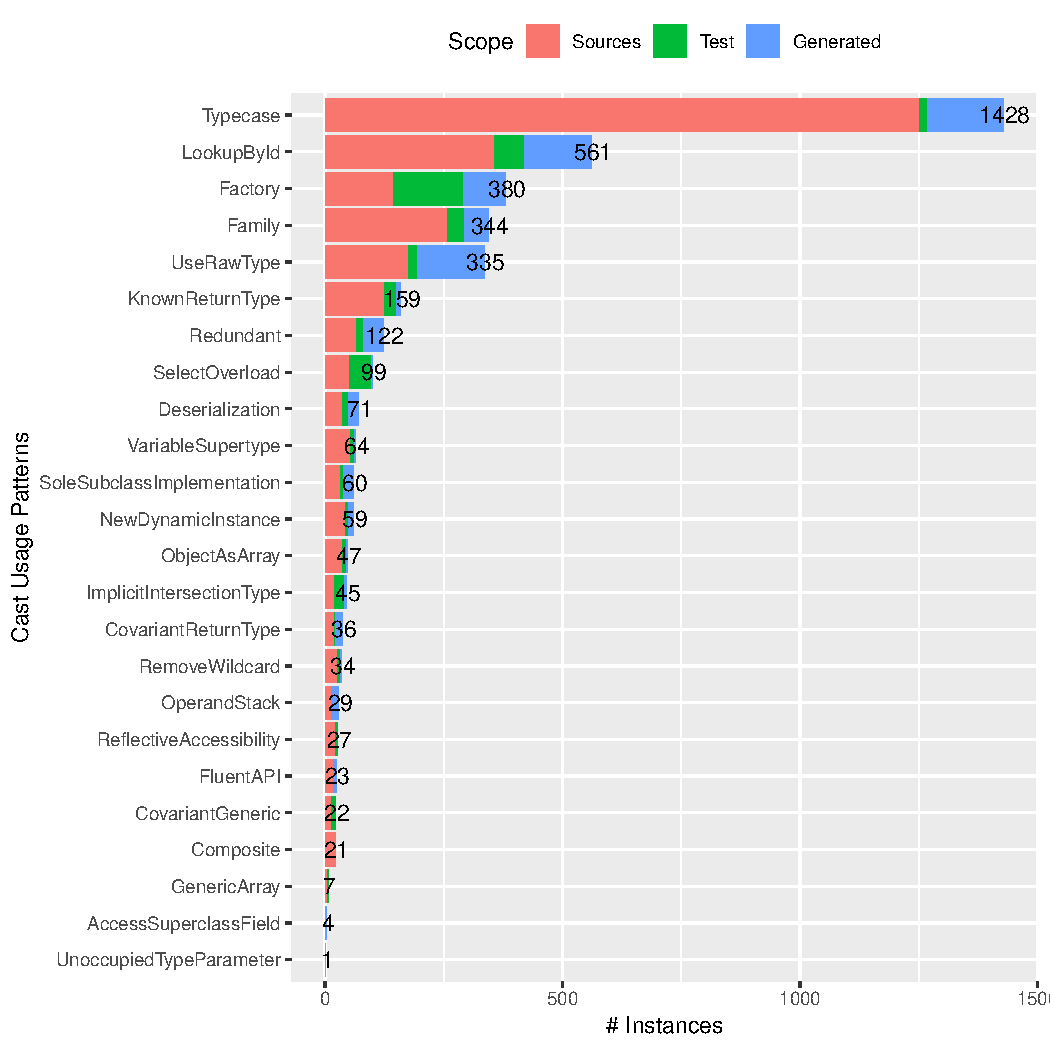
\includegraphics[width=\textwidth]{analysis/table-patterns.pdf}
\caption{Cast Pattern Occurrences} \label{fig:patterns}
\end{figure}

\discuss{Matthias: Start a new subsection here.}
\done{Matthias: When describing each pattern, you may want to repeat the number of occurrences within the description {\scriptsize (maybe as part of the section title, or just below)}}
Each pattern is described using the following template:

\begin{itemize}
\item \textbf{Description.}
Tells what the pattern is about.
It gives a general overview of the structure of the pattern.
\item \textbf{Instances.}
Gives one or more concrete examples found in real code.
%
\done{Nate: What's the orange (hightlight color) mean? The line with the cast being inspected. Explain here}
%
Each example contains a highlighted line which shows the cast instance being inspected.
Please notice that the snippets presented here were slightly
modified for formatting purposes.
Moreover, to facilitate some snippet presentations,
we remove irrelevant code and replace it with the
comment \code{// [...]}.
For each instance presented here, we provide the link to the source code repository in \lgtm{}.
We provide the link in case the reader wants to do further inspection
of the presented snippet.
%
\done{Nate: List project name too.}
%
Instead of presenting \lgtm{} long URLs,
we have used the URL shortening service
\href{https://bitly.com/}{\bitly} for easier reading.
%
\done{Luis: Links were customized to include the project names.}
%
Each \bitly{} link was customized to include the project name.
\item \textbf{Detection.}
Describes briefly how this pattern was detected in terms of the tags introduced in the previous section.
\item \textbf{Discussion.}
Presents suggestions, flaws, or comments about the pattern.
\item \textbf{Related Patterns.}
%
\done{Nate: Remove "?"}
%
How the pattern being described relates to other patterns.
\end{itemize}

\group{Language Designers}

\done{Matthias: Say what it means to be guarded.}
The patterns in this category are guarded casts.
A guarded cast is a cast such that before the cast is applied,
some condition --- the \emph{guard} -- needs to be verified.
The condition to be verified guarantees that the cast will not fail at runtime (unless there is a bug in the application), \ie,
the cast will not throw a \code{ClassCastException}.
Some kind of guards ensure that the cast will not fail at the language-level,
while others only can guarantee it at the application-level.

\group{Tool Builders1}

\done{Matthias: In these paragraphs, can you also enumerate the patterns by name, so readers see what's coming?}
\done{Matthias: ???}
Creational patterns are cast instances that are determined by how the value being cast is created.

\group{Developers}

These patterns can be avoidable either directly (by removing them)
or through some minor refactor.
Some of these patterns in this category also are 
These are code smells.

\begin{pattern}{Typecase}
The \thisp{} pattern consists of dispatching to different cases
depending on the run-time type of the source value.
The run-time type is tested against known subtypes of the operand type,
with each test followed by a cast to that type.
The guard may be implemented using one of three variants:
an \code{instanceof} operator (\variant{GuardByInstanceOf}),
a comparison of the runtime class against a class literal (\variant{GuardByClassLiteral}),
or an application-specific type tag (\variant{GuardByTypeTag}).

\instances{}
\thisp{} is by far the most common pattern.
Figure~\ref{fig:casts:typecase} shows the different variants of the pattern.
The \variant{GuardByInstanceOf} is the most used variant.
Often there is just one case and the default case, \ie,
when the guard fails, performs a no-op or reports an error.

\plot{patterns/table-pattern-Typecase-features}{fig:casts:typecase}{\thisp{} Variant Occurrences}

The following listing shows an example of the \thisp{} pattern,
using the \variant{GuardByInstanceOf} variant.

%https://lgtm.com/projects/g/PenguinSquad/Enchiridion/snapshot/dist-19218583-1524814812150/files/build/sources/main/java/joshie/enchiridion/helpers/StackHelper.java?sort=name&dir=ASC&mode=heatmap#L27
\def\urlvar{http://bit.ly/PenguinSquad_Enchiridion_2HnNwB7}
\begin{minted}[highlightlines=6]{java}
if (object instanceof Item) {
	return getStringFromStack(new ItemStack((Item) object));
} else if (object instanceof Block) {
	return getStringFromStack(new ItemStack((Block) object));
} else if (object instanceof ItemStack) {
	return getStringFromStack((ItemStack) object);
} else if (object instanceof String) {
	return (String) object;
} else if (object instanceof List) {
	return getStringFromStack((ItemStack) ((List) object).get(0));
} else return ""; #\urlbox#
\end{minted}

In the next case a type test is performed---through a method call---before actually applying the cast to the variable \code{props} (line 3).
Note that the type test is internally using the \code{instanceof} operator (line 8).

%https://lgtm.com/projects/g/apache/poi/snapshot/dist-1790760597-1524814812150/files/src/ooxml/java/org/apache/poi/xslf/usermodel/XSLFPropertiesDelegate.java?sort=name&dir=ASC&mode=heatmap#L1367
\def\urlvar{http://bit.ly/apache_poi_2FW5SXU}
\begin{minted}[highlightlines=3]{java}
@Override
public CTSolidColorFillProperties getSolidFill() {
    return isSetSolidFill() ? (CTSolidColorFillProperties) props : null;
}
@Override
public boolean isSetSolidFill() {
    return (props instanceof CTSolidColorFillProperties);
} #\urlbox#
\end{minted}

Another common scenario is when several cases are used to re-\code{throw}
an exception of the right type, as shown below.
The cast instance is applied to a variable of type \code{Throwable}
(line 13).
Nevertheless, the enclosing method is only allowed to throw \code{NamingException} by the \code{throws} declaration (line 3).
Since an exception of type \code{Throwable} is checked,
a cast to \code{VirtualMachineError} (subclass of \code{Error}) is needed.

%https://lgtm.com/projects/g/codefollower/Tomcat-Research/snapshot/dist-13734061-1524814812150/files/java/org/apache/naming/factory/DataSourceLinkFactory.java?sort=name&dir=ASC&mode=heatmap#L85
\def\urlvar{http://bit.ly/codefollower_Tomcat_Research_2SGDUG5}
\begin{minted}[highlightlines=13]{java}
protected Object wrapDataSource(
			Object datasource, String username, String password)
			throws NamingException {
	try {
		// [...]
	}catch (Exception x) {
		if (x instanceof InvocationTargetException) {
			Throwable cause = x.getCause();
			if (cause instanceof ThreadDeath) {
				throw (ThreadDeath) cause;
			}
			if (cause instanceof VirtualMachineError) {
				throw (VirtualMachineError) cause;
			}
			if (cause instanceof Exception) {
				x = (Exception) cause;
			}
		}
		if (x instanceof NamingException) throw (NamingException)x;
		else {
			// [...]
		}
	}
} #\urlbox#
\end{minted}

The next example shows that \thisp{} can also be used to filter elements by type within a stream.
The cast is applied to stream operations (line 1) over the \code{caseAssignments} collection.
The \code{instanceof} guard is tested in line 2.

%https://lgtm.com/projects/g/kiegroup/jbpm/snapshot/dist-1810050-1524814812150/files/jbpm-case-mgmt/jbpm-case-mgmt-impl/src/main/java/org/jbpm/casemgmt/impl/wih/StartCaseWorkItemHandler.java?sort=name&dir=ASC&mode=heatmap#L212
\def\urlvar{http://bit.ly/kiegroup_jbpm_2ENCL8a}
\begin{minted}[highlightlines=1-4]{java}
user = (User) caseAssignments
                .stream().filter(oe -> oe instanceof User)
                .findFirst()
                .orElseThrow(() -> new IllegalArgumentException());
#\urlbox#
\end{minted}

Rather than using an \code{instanceof} guard, in the following example
the target type of the parameter \code{reference} is determined by the value
of the parameter \code{referenceType},
which acts as a \emph{type tag} for \code{reference}.

%https://lgtm.com/projects/b/JesusFreke/smali/snapshot/dist-1306230039-1524814812150/files/dexlib2/src/main/java/org/jf/dexlib2/writer/InstructionWriter.java?sort=name&dir=ASC&mode=heatmap#L492
\def\urlvar{http://bit.ly/JesusFreke_smali_2Ho8bVL}
\begin{minted}[highlightlines=7]{java}
switch (referenceType) {
    case ReferenceType.FIELD:
        return fieldSection.getItemIndex((FieldRefKey) reference);
    case ReferenceType.METHOD:
        return methodSection.getItemIndex((MethodRefKey) reference);
    case ReferenceType.STRING:
        return stringSection.getItemIndex((StringRef) reference);
    case ReferenceType.TYPE:
        return typeSection.getItemIndex((TypeRef) reference);
    case ReferenceType.METHOD_PROTO:
        return protoSection.getItemIndex((ProtoRefKey) reference);
    default:
        throw new ExceptionWithContext("/* [...] */", referenceType);
} #\urlbox#
\end{minted}

In some cases, the target types of the casts are the same in every branch.
In the following snippet,
the cast is applied to the \code{message.obj} field to (line 11),
according to the value of the tag \code{message.what} field (line 1).
However, a similar cast is applied in the first branch (line 3).
In both branches \code{message.obj} is of type \code{Object[]},
but with different lengths.
The casts in the calls to \code{onSuccess} and
\code{onFailure} (lines 5, 13--14)
are instances of the \nameref{pat:ObjectAsArray} pattern.

%https://lgtm.com/projects/g/loopj/android-async-http/snapshot/dist-1879340034-1549372228293/files/library/src/main/java/com/loopj/android/http/AsyncHttpResponseHandler.java?sort=name&dir=ASC&mode=heatmap#L359
\def\urlvar{http://bit.ly/loopj_android_async_http_2IpIULk}
\begin{minted}[highlightlines=10]{java}
switch (message.what) {
    case SUCCESS_MESSAGE:
        response = (Object[]) message.obj;
        if (response != null && response.length >= 3) {
            onSuccess((Integer) response[0], (Header[]) response[1],
					(byte[]) response[2]);
        } else { /* [...] */ }
        break;
    case FAILURE_MESSAGE:
        response = (Object[]) message.obj;
        if (response != null && response.length >= 4) {
            onFailure((Integer) response[0], (Header[]) response[1],
                    (byte[]) response[2], (Throwable) response[3]);
        } else { /* [...] */ }
        break;
    // [...]
} #\urlbox#
\end{minted}

In the next example, instead of a \code{switch},
an \code{if} statement is used to guard the cast (in line 6).

%https://lgtm.com/projects/g/FenixEdu/fenixedu-academic/snapshot/dist-29270029-1524814812150/files/src/main/java/org/fenixedu/academic/ui/renderers/student/curriculum/StudentCurricularPlanRenderer.java?sort=name&dir=ASC&mode=heatmap#L853
\def\urlvar{http://bit.ly/FenixEdu_fenixedu_academic_2SUNOUJ}
\begin{minted}[highlightlines=6]{java}
for (final IEnrolment enrolment : dismissal.getSourceIEnrolments()) {
    if (enrolment.isExternalEnrolment()) {
        generateExternalEnrolmentRow(mainTable, (ExternalEnrolment) enrolment,
                level + 1, true);
    } else {
        generateEnrolmentRow(mainTable, (Enrolment) enrolment,
                level + 1, false, true, true);
    }
} #\urlbox#
\end{minted}

In the next example,
the parameter \code{args} is cast to \code{Object[]} (line 13).
The ``type tag'' is given by the fact that the cast is executed in a \code{catch} block,
and that \code{value} is an instance of \code{Closure} (line 9).
The \code{args} parameter flows into two methods,
\code{invokeMethod(String name, Object args)} and
\code{call(Object... args)}.
Thus, \code{args} is treated as an \code{Object} or \code{Object[]} depending on the type tag, resembling an union type.

%https://lgtm.com/projects/g/groovy/groovy-core/snapshot/dist-45390050-1524814812150/files/src/main/groovy/util/Expando.java?sort=name&dir=ASC&mode=heatmap#L103
\def\urlvar{http://bit.ly/groovy_groovy_core_2SGzK16}
\begin{minted}[highlightlines=13]{java}
public Object invokeMethod(String name, Object args) {
    try {
        return super.invokeMethod(name, args);
    }
    catch (GroovyRuntimeException e) {
        // br should get a "native" property match first.
        // getProperty includes such fall-back logic
        Object value = this.getProperty(name);
        if (value instanceof Closure) {
            Closure closure = (Closure) value;
            closure = (Closure) closure.clone();
            closure.setDelegate(this);
            return closure.call((Object[]) args);
        } else {
            throw e;
        }
    }
} #\urlbox#
\end{minted}

In the \variant{GuardByClassLiteral} variant, a cast uses an application-specific guard, but the guard depends on a class literal.
In the following example,
a cast is performed to the \code{field} variable (line 22),
based whether the runtime class of the variable is actually \code{Short.class}.

%https://lgtm.com/projects/g/elastic/elasticsearch/snapshot/dist-1916470085-1524814812150/files/server/src/main/java/org/elasticsearch/common/lucene/Lucene.java?sort=name&dir=ASC&mode=heatmap#L478
\def\urlvar{http://bit.ly/elastic_elasticsearch_2SSgsFV}
\begin{minted}[highlightlines=22]{java}
Class type = field.getClass();
if (type == String.class) {
    out.writeByte((byte) 1);
    out.writeString((String) field);
} else if (type == Integer.class) {
    out.writeByte((byte) 2);
    out.writeInt((Integer) field);
} else if (type == Long.class) {
    out.writeByte((byte) 3);
    out.writeLong((Long) field);
} else if (type == Float.class) {
    out.writeByte((byte) 4);
    out.writeFloat((Float) field);
} else if (type == Double.class) {
    out.writeByte((byte) 5);
    out.writeDouble((Double) field);
} else if (type == Byte.class) {
    out.writeByte((byte) 6);
    out.writeByte((Byte) field);
} else if (type == Short.class) {
    out.writeByte((byte) 7);
    out.writeShort((Short) field);
} else if (type == Boolean.class) {
    out.writeByte((byte) 8);
    out.writeBoolean((Boolean) field);
} else if (type == BytesRef.class) {
    out.writeByte((byte) 9);
    out.writeBytesRef((BytesRef) field);
} else {
    throw new IOException("Can't handle sort field value of type ["+type+"]");
} #\urlbox#
\end{minted}

Similar to the previous example, the next snippet contains several type cases.
Each type case is guarded by an \code{equals} comparison between a class literal and the \code{clazz} parameter.
The cast is applied to the type parameter \code{T} only if the guard succeeds.

%https://lgtm.com/projects/g/OPCFoundation/UA-Java-Legacy/snapshot/dist-1804064538-1524814812150/files/src/main/java/org/opcfoundation/ua/encoding/binary/BinaryDecoder.java?sort=name&dir=ASC&mode=heatmap#L214
\def\urlvar{http://bit.ly/OPCFoundation_UA_Java_Legacy_2Fb2xmZ}
\begin{minted}[highlightlines=9]{java}
@Override
@SuppressWarnings("unchecked")
public <T> T get(String fieldName, Class<T> clazz) throws DecodingException {
    if (clazz.equals(Boolean.class)) {
        return (T) getBoolean(fieldName);
    }
    // [...]
    if (clazz.equals(ExtensionObject.class)) {
        return (T) getExtensionObject(fieldName);
    }
    // [...]
} #\urlbox#
\end{minted}

In the following listing,
a cast is applied to the result of the \code{getObject} method (line 2).
The target type of the cast, \code{MyKey}, corresponds to the class literal argument, \code{MyKey.class}.
Essentially, \code{getObject} is using the \code{isInstance} method%
\footnote{\url{https://docs.oracle.com/javase/8/docs/api/java/lang/Class.html\#isInstance-java.lang.Object-}}
of the class \code{java.lang.Class} to check whether an object is from a certain type.

%https://lgtm.com/projects/g/smartdevicelink/sdl_android/snapshot/dist-2037360569-1524814812150/files/sdl_android/src/main/java/com/smartdevicelink/proxy/rpc/GetVehicleDataResponse.java?sort=name&dir=ASC&mode=heatmap#L236
\def\urlvar{http://bit.ly/smartdevicelink_sdl_android_2EjJiaq}
\begin{minted}[highlightlines=2]{java}
public MyKey getMyKey() {
    return (MyKey) getObject(MyKey.class, KEY_MY_KEY);
} #\urlbox#
\end{minted}

The following snippet shows an instance of the \variant{GuardByClassLiteral} variant. 
In this case, the cast is guaranteed to succeed because the class literal used as argument to the recursive call (\code{Integer.class}) determines that the method returns an \code{int} value.
%https://lgtm.com/projects/g/apache/karaf/snapshot/dist-13960098-1524814812150/files/shell/core/src/main/java/org/apache/karaf/shell/support/converter/DefaultConverter.java?sort=name&dir=ASC&mode=heatmap#L117
\def\urlvar{http://bit.ly/apache_karaf_2HE55gE}
\begin{minted}[highlightlines=4]{java}
public Object convertToNumber(Number value, Class toType) throws Exception {
    toType = unwrap(toType);
    if (AtomicInteger.class == toType) {
        return new AtomicInteger((Integer)convertToNumber(value,Integer.class));
    } else if (AtomicLong.class == toType) {
        return new AtomicLong((Long) convertToNumber(value, Long.class));
    } else if (Integer.class == toType) {
        return value.intValue();
    } else if (Short.class == toType) {
        return value.shortValue();
    } else if (Long.class == toType) {
        return value.longValue();
    } else if (Float.class == toType) {
        return value.floatValue();
    } else if (Double.class == toType) {
        return value.doubleValue();
    } else if (Byte.class == toType) {
        return value.byteValue();
    } else if (BigInteger.class == toType) {
        return new BigInteger(value.toString());
    } else if (BigDecimal.class == toType) {
        return new BigDecimal(value.toString());
    } else {
        throw new Exception("Unable to convert number "+value+" to "+toType);
    }
} #\urlbox#
\end{minted}


\detection{}
When implementing the pattern,
care must be taken with complex operands that the value of the operand is
not changed between the guard and the cast, possibly even by another thread.
For instance, in some situations the operand expression is a method invocation.
The value returned by the method should be the same for both the
\code{instanceof} and the cast, thus the method should be a pure method.
Typically, this problem is avoided by using an effectively final local variable in both the guard and the cast operand.

The Query~\ref{lst:ql:GuardByInstanceOfCast} detects the \variant{GuardByInstanceOf} variant.
It is decoupled in two \ql{} classes.
The \code{ControlByInstanceOfCast} class checks that the cast---\emph{to a variable}---is control-dependant on a \code{instanceof} on the same variable.
Then, the \code{GuardByInstanceOfCast} class checks that the value tested by the \code{instanceof} is the same to be cast.
That is, it checks that there is no assignment to the variable between the \code{instanceof} and the cast.

\begin{listing}
\begin{minted}{java}
class ControlByInstanceOfCast extends #\qlref{VarCast}# { #\qlbox#
	InstanceOfExpr iof;
	private ConditionBlock cb;
	ControlByInstanceOfCast() {
		iof = cb.getCondition() and
		cb.controls(getBasicBlock(), true) and
		var.getAnAccess() = iof.getExpr()
	}
	InstanceOfExpr getIof() { result = iof }
}

class GuardByInstanceOfCast extends ControlByInstanceOfCast {
	GuardByInstanceOfCast() {
		forall (VariableUpdate def | defUsePair(def, getExpr()) |
		  defUsePair(def, iof.getExpr())
		)
	}
}
\end{minted}
\caption{Query for the \variant{GuardByInstanceOf} variant.}
\label{lst:ql:GuardByInstanceOfCast}
\end{listing}

The implementation of \variant{GuardByTypeTag} variant is application-specific,
and thus its automatic detection in \ql{} is impractical.
Nevertheless, the Query~\ref{lst:casts:detect:switchtypetag} detect the special case when a cast is applied to a field in an object inside a \code{switch} statement.
The expression to be \code{switch}ed is another field in the same object.

\begin{listing}
\begin{minted}{java}
class SwitchFieldTypeTagCast extends #\qlref{Cast}# { #\qlbox#
	FieldAccess tagAccess;
	FieldAccess castAccess;
	Variable v;
	SwitchFieldTypeTagCast() {
		tagAccess = this.(SwitchedExpr).getSwitchStmt().getExpr() and
		castAccess = getExprOrDef() and
		v.getAnAccess() = tagAccess.getQualifier() and
		v.getAnAccess() = castAccess.getQualifier()
	}
}
\end{minted}
\caption{Detection of a cast inside a \code{switch} statement}
\label{lst:casts:detect:switchtypetag}
\end{listing}

Similar to the previous case,
the Query~\ref{lst:casts:detect:isarraytypetag} detects when a cast is guarded by a call to the \code{Class.isArray} method.
This query detects \emph{only} the case when the variable to be cast and
the \code{getClass} invocation are in the same method.

\begin{listing}
\begin{minted}{java}
class ControlByIsArrayCast extends #\qlref{VarCast}# { #\qlbox#
	ConditionBlock cb;
	MethodAccess iama;
	ControlByIsArrayCast() {
		exists (VariableAssign def, GetClassMethodAccess gcls |
			gcls.getQualifier() = var.getAnAccess() and
			def.getSource() = gcls and
			defUsePair(def, iama.getQualifier().(VarAccess) )
		) and
		iama.getMethod() instanceof IsArrayClassMethod and
		(
			(cb.getCondition()=iama and cb.controls(getBasicBlock(), true)) or
			(cb.getCondition().(LogNotExpr).getExpr() = iama and
				cb.controls(getBasicBlock(), false)
			)
		)
	}
}
\end{minted}
\caption{Detection of a cast guarded by the \code{Class.isArray} method.}
\label{lst:casts:detect:isarraytypetag}
\end{listing}

The following query detects the \variant{GuardByClassLiteral} variant.
Similar to the previous case,
this query \emph{does not} detect the case when the variable to be cast and the \code{Class} object are passed as parameters.
To detect such case would require an inter-procedural (global) data flow analysis.
Such analysis does not scale easily.

\begin{listing}
\begin{minted}{java}
class GuardByClassLiteral extends #\qlref{VarCast}# { #\qlbox#
	TypeLiteral tl;
	GetClassMethodAccess gcma;
	GuardByClassLiteral() {
		gcma.getQualifier() = getVar().getAnAccess() and
		#\qlref{isSubtype}#(tl.getTypeName().getType(), getTargetType()) and (
			#\qlref{controlByEqualityTest}#(tl, gcma, this) or
			#\qlref{controlByEqualsMethod}#(tl, gcma, this)
		)
	}
}
\end{minted}
\caption{Query for the \variant{GuardByClassLiteral} variant.}
\end{listing}


\issues{}
Having only a single case---that is, a single guard and cast---is common.
In the 742 instances of \thisp{} that used \code{instanceof}, 511
(69\%) had only one case.

The \thisp{} pattern can be seen as an \adhoc{} alternative to a
\code{typecase} or pattern matching~\citep{milnerProposalStandardML1984} as a
language construct.
In \kotlin{}, flow-sensitive typing is used so that immutable values can be
used at a subtype when a type guard on the value is successful.%
\footnote{\url{https://kotlinlang.org/docs/reference/typecasts.html\#smart-casts}}
This feature eliminates much of the need for the guarded casts.
Pattern matching can be seen in several other languages, \eg, \ml{}, \scala{}, \csharp{}, and \haskell{}.
For instance, in \scala{} the pattern matching construct is achieved using the \code{match} keyword.
In this example,%
\footnote{Adapted from \url{https://docs.scala-lang.org/tour/pattern-matching.html}}
a different action is taken according to the runtime type of the parameter \code{notification} (line 10).

\begin{minted}[highlightlines=10]{scala}
abstract class Notification #\scalabox#
case class Email(sender: String, title: String, body: String)
	extends Notification
case class SMS(caller: String, message: String)
	extends Notification
case class VoiceRecording(contactName: String, link: String)
	extends Notification

def showNotification(notification: Notification): String = {
	notification match {
		case Email(email, title, _) => s"Email from $email titled: $title"
		case SMS(number, message) => s"SMS from $number! Message: $message"
		case VoiceRecording(name, link) => s"Recording from $name! Link: $link"
	}
}
\end{minted}

Alternatives to the \thisp{} pattern would be to use the visitor pattern or to use virtual dispatch on the match scrutinee.
However, both of these alternatives might be difficult to implement when the scrutinee is defined in a library or in third-party code.
There is an ongoing proposal%
\footnote{\url{https://openjdk.java.net/jeps/305}}$^{,}$%
\footnote{\url{https://cr.openjdk.java.net/~briangoetz/amber/pattern-match.html}}%
~\citep{jep305} to add pattern matching to the \java{} language.
The proposal explores changing the \code{instanceof} operator in order to support pattern matching.
\java{} 12 extends the \code{switch} statement to be used as either a statement or an expression%
\footnote{\url{https://openjdk.java.net/jeps/325}}$^{,}$%
\footnote{\url{https://openjdk.java.net/jeps/354}}~\citep{jep325,jep354}.
This enhancement aims to ease the transition to a \code{switch} expression that supports pattern matching.

The \variant{GuardByClassLiteral} variant may be used instead of the \code{instanceof} operator when the developer wants to match exactly the runtime class of an object.
The \code{instanceof} operator%
\footnote{\url{https://docs.oracle.com/javase/specs/jls/se8/html/jls-15.html\#jls-15.20.2}}
returns \code{true} if the expression could be cast to the specified type,
whereas using a class literal comparison returns \code{true} if the expression is exactly the runtime class.

In some cases, the \variant{GuardByTypeTag} variant can be replaced by \variant{GuardByInstanceOf}.
However, if the application-specific tag is a numeric value,
the \variant{GuardByTypeTag} could perform better than the \variant{GuardByInstanceOf} using \code{instanceof}.
Moreover, there are situation where the \code{instanceof} operator cannot be avoid since the types to be cast are the same.

\end{pattern}

\begin{pattern}{LookupById}
This pattern is used to extract values from a heterogenous container.
It looks up an object by a compile-time constant identifier, tag, or name and casts the result to an appropriate type.
It accesses a collection that holds values of different types
(usually implemented as \code{Collection<Object>} or as \code{Map<K, Object>}).
The actual run-time type returned from the lookup is determined by the value of the identifier.

\instances{}
In the example shown below,%
\footnote{\url{http://bit.ly/loopj_android-async-http_2SUzY4E}}
the \code{getAttribute} method returns \code{Object}.
The variable \texttt{context} is of type \code{BasicHttpContext},
which is implemented with \code{HashMap}.

%https://lgtm.com/projects/g/loopj/android-async-http/snapshot/dist-1879340034-1518514025554/files/library/src/main/java/com/loopj/android/http/AsyncHttpClient.java?sort=name&dir=ASC&mode=heatmap&excluded=false#L258
\begin{minted}[highlightlines=1,linenos=false]{java}
AuthState authState = (AuthState) context.getAttribute(ClientContext.TARGET_AUTH_STATE);
\end{minted}

The next snippet%
\footnote{\url{http://bit.ly/skerit_cmusphinx_2HGgL1D}}
shows a call site to the \code{getComponent} method cast to the \code{ActiveListManager} class (line 15).
The \code{getComponent} method in this cast instance uses as argument the \code{PROP\_ACTIVE\_LIST\_MANAGER} constant.
Looking at the definition of this constant (line 3),
we can see there is a companion attribute (\code{@S4Component}) whose argument is the \code{ActiveListManager} class, the target of the cast instance.

% https://lgtm.com/projects/g/skerit/cmusphinx/snapshot/dist-1506204046584-1524814812150/files/sphinx4/src/sphinx4/edu/cmu/sphinx/decoder/search/WordPruningBreadthFirstSearchManager.java?sort=name&dir=ASC&mode=heatmap#L207
\begin{minted}[highlightlines=15]{java}
/** The property that defines the type of active list to use */
@S4Component(type = ActiveListManager.class)
public final static String PROP_ACTIVE_LIST_MANAGER = "activeListManager";

@Override
public void newProperties(PropertySheet ps) throws PropertyException {
    super.newProperties(ps);
    logMath = (LogMath) ps.getComponent(PROP_LOG_MATH);
    logger = ps.getLogger();
    linguist = (Linguist) ps.getComponent(PROP_LINGUIST);
    pruner = (Pruner) ps.getComponent(PROP_PRUNER);
    scorer = (AcousticScorer) ps.getComponent(PROP_SCORER);
    activeListManager = 
            (ActiveListManager) ps.getComponent(PROP_ACTIVE_LIST_MANAGER);
    // [...]
}
\end{minted}

A common version of this pattern is to retrieve a value instantiated from
static resource file, \eg,
an XML, HTML or \java{} properties file.
The file contents are (in theory) known at compile-time and the file is included in the binary distribution
of the application. These files are often built using tools such as GUI
builders.

In the following example from an Android application,%
\footnote{\url{http://bit.ly/pwittchen_NetworkEvents_2HGbrMq}}
a cast is applied to the \code{findViewById} method invocation.
View classes are instantiated by the application framework using an XML resource file.
The \code{findViewById} method looks up the view by its ID.

%https://lgtm.com/projects/g/pwittchen/NetworkEvents/snapshot/dist-2032650416-1524814812150/files/example/src/main/java/com/github/pwittchen/networkevents/app/MainActivity.java?sort=name&dir=ASC&mode=heatmap#L65
\begin{minted}[highlightlines=1,linenos=false]{java}
mobileNetworkType = (TextView) findViewById(R.id.mobile_network_type);
\end{minted}

\discussion{}
This pattern suggests a heterogeneous dictionary.
In our manual inspection,
all dictionary keys and the resulting types are known at
compile time, however
a cast is needed because the dictionary type does not encode the
relationship between key values and the result type.
Casts in this pattern are typically not guarded indicating that the programmer
knows the source of the cast based on the value of the key.

This pattern is often seen in Android applications.
The Butter Knife framework%
\footnote{\url{http://jakewharton.github.io/butterknife/}}
uses annotations to avoid the ``manual'' casting.
Instead, code is generated that casts the result of \code{findViewById} to the
appropriate type.


But in any case a cast is needed given the inexpressiveness of the type system.
As a complementary analysis,
it would be interesting to check whether all call sites to
\code{getAttribute} receives a constant (\code{final static} field).

Notice that this pattern is not guarded by an \code{instanceof}.
However, the cast involved does not fail at runtime.
This means that the source of the cast is known to the programmer.
This raises the following questions:
\begin{itemize}
\item \emph{What kind of analysis is needed to detect the source of the cast?}
\item \emph{Is worth to have it?}
\item \emph{Is better to change API?}
\item \emph{How other --- statically typed --- languages support this kind of idiom?}
\item \emph{Could generative programming a.k.a. templates solve this problem?}
\end{itemize}

This pattern retrieves a stashed a value from an heterogeneous collection (or dictionary).
A cast is needed because the return type depends on the ID to be retrieved.
This scenario is similar to the \nameref{pat:Tag} pattern,
where usually the developer retrieves a stashed value from a superclass field.
Since this pattern casts a value to a known type from a method invocation,
it can be seen as a kind of \nameref{pat:KnownReturnType} pattern.

\end{pattern}
\begin{pattern}{Factory}
Creates an object based on some arguments to a method call.
Since the arguments are known at compile-time, cast to the specific type.
In this pattern, the arguments resemble a ``type tag'' descriptor (cf.
\nameref{pat:Typecase}).

This pattern is characterized by a cast to a method call passing one or more arguments.
The method call needs to create an object based on those arguments.
Usually the arguments that determine the run-time type to be returned are known at compile-time.

\instances{}
The following snippet
shows an instance of the \thisp{} pattern.
The cast is applied to the result of invoking \code{keyPair.get\-Private}
(line 6).
The variable \code{keyPair} is assigned the result of \code{pairGen.\-generateKeyPair} (line 3).
At the same time, the \code{pairGen} variable is assigned the value returned by \code{KeyPairGenerator.getInstance("RSA")}.
The argument \code{"RSA"} indicates the algorithm to use.
The method%
\footnote{\url{https://docs.oracle.com/javase/8/docs/api/java/security/KeyPair.html\#getPrivate()}}
will return a reference to the private key component,
and this is determined by the algorithm argument described above.

%https://lgtm.com/projects/b/connect2id/oauth-2.0-sdk-with-openid-connect-extensions/snapshot/dist-1311020143-1524814812150/files/src/test/java/com/nimbusds/oauth2/sdk/jose/jwk/RemoteJWKSetTest.java?sort=name&dir=ASC&mode=heatmap#L242
\def\urlvar{http://bit.ly/connect2id_oauth_2_0_sdk_with_2HvRlUX}
\begin{minted}[highlightlines=6]{java}
KeyPairGenerator pairGen = KeyPairGenerator.getInstance("RSA");
pairGen.initialize(1024);
KeyPair keyPair = pairGen.generateKeyPair();
// [...]
RSAKey rsaJWK2 = new RSAKey.Builder((RSAPublicKey) keyPair.getPublic())
        .privateKey((RSAPrivateKey) keyPair.getPrivate())
        .keyID("2")
        .build(); #\urlbox#
\end{minted}

Similar to the above snippet,
the next example shows an instance of this pattern where a cast is performed on the result of the \code{openConnection} method%
\footnote{\url{https://docs.oracle.com/javase/8/docs/api/java/net/URL.html\#openConnection--}}
(line 2).
The method is declared to return \code{URLConnection} but can return a more specific type based on the URL string.
The \code{openConnection} method is applied to the \code{url} variable,
which is assigned in line 1 using the \code{URL} constructor.
The argument to the constructor is an \code{http} URL,
thus the result is cast to \code{HttpURLConnection}.
%https://lgtm.com/projects/g/apache/hadoop/snapshot/dist-956730001-1524814812150/files/hadoop-yarn-project/hadoop-yarn/hadoop-yarn-server/hadoop-yarn-server-resourcemanager/src/test/java/org/apache/hadoop/yarn/server/resourcemanager/webapp/TestRMWebServicesHttpStaticUserPermissions.java?sort=name&dir=ASC&mode=heatmap#L138
\def\urlvar{http://bit.ly/apache_hadoop_2E6KY6T}
\begin{minted}[highlightlines=2]{java}
URL url = new URL("http://localhost:8088/ws/v1/cluster/apps");
HttpURLConnection conn = (HttpURLConnection) url.openConnection();
#\urlbox#
\end{minted}

The following example shows how a cast (line 3) is being determined by the argument to the \code{CertificateFactory.getInstance} method (line 1).
The argument is the string \code{"X.509"},
therefore the method \code{generateCRL} will return a value of type \code{X509CRL}.

%https://lgtm.com/projects/g/bcgit/bc-java/snapshot/dist-20740003-1524814812150/files/prov/src/test/java/org/bouncycastle/jce/provider/test/X509LDAPCertStoreTest.java?sort=name&dir=ASC&mode=heatmap#L241
\def\urlvar{http://bit.ly/bcgit_bc_java_2TEVScM}
\begin{minted}[highlightlines=3]{java}
CertificateFactory cf = CertificateFactory.getInstance("X.509", "BC");
// [...]
X509CRL crl = (X509CRL)cf.generateCRL(new ByteArrayInputStream(directCRL));
#\urlbox#
\end{minted}

In our last example the cast instance (line 2) is applied to the result of \code{parse} method.
The return type of \code{parse} is of type \code{Statement}, but,
since the statement is a \code{SELECT} statement,
the value returned by the \code{parse} method is known to be of type \code{Select}
and the cast should succeed.
%https://lgtm.com/projects/g/JSQLParser/JSqlParser/snapshot/dist-43250114-1524814812150/files/src/test/java/net/sf/jsqlparser/test/select/SelectTest.java?sort=name&dir=ASC&mode=heatmap#L437
\def\urlvar{http://bit.ly/JSQLParser_JSqlParser_2TecMyB}
\begin{minted}[highlightlines=2]{java}
statement = "SELECT * FROM mytable WHERE mytable.col = 9 LIMIT :param_name";
select = (Select) parserManager.parse(new StringReader(statement));
public class Select implements Statement {
        // [...]
}
public class CCJSqlParserManager implements JSqlParser {
    @Override
    public Statement parse(Reader statementReader) throws JSQLParserException {
        // [...]
    }
} #\urlbox#
\end{minted}

In some cases of this pattern, a cast is applied to a method invocation where one of its arguments is a class literal.
The target type of the cast is determined by this class literal,
like in the following snippets.
%https://lgtm.com/projects/g/liferay/liferay-ide/snapshot/dist-2980259-1524814812150/files/tools/plugins/com.liferay.ide.server.ui/src/com/liferay/ide/server/ui/handlers/RedeployHandler.java?sort=name&dir=ASC&mode=heatmap#L64
\def\urlvar{http://bit.ly/liferay_liferay_ide_2FMG0f6}
\begin{minted}[highlightlines=2-3]{java}
final ILiferayServerBehavior liferayServerBehavior =
                (ILiferayServerBehavior) moduleServer.getServer()
                        .loadAdapter( ILiferayServerBehavior.class, null );
#\urlbox#
\end{minted}

%https://lgtm.com/projects/g/robovm/robovm/snapshot/dist-39650108-1524814812150/files/cocoatouch/src/main/java/org/robovm/apple/corevideo/CVBufferMovieTime.java?sort=name&dir=ASC&mode=heatmap#L66
\def\urlvar{http://bit.ly/robovm_robovm_2FMFWvS}
\begin{minted}[highlightlines=1]{java}
CFArray o = (CFArray) CFType.Marshaler.toObject(CFArray.class, handle, flags);
#\urlbox#
\end{minted} 


\detection{}
The detection of this pattern requires to analyse the factory method being called.
This is not always possible in \ql{},
since \ql{} does not analyse project dependencies.

In several instances, to manually determine when a cast belongs to this pattern,
we had to look-up the method implementation in external source code repositories.

\issues{}
In some situations, the use of this pattern can be seen as breaking the contract \api{} between the caller and the callee.
This happens because the caller needs to know how the method is implemented in order to determine the run-time return type.
In \thisp{}, there is a known type hierarchy 
below the return type and the caller casts to a known subtype
in that hierarchy based on the arguments passed into the factory method.

The \nameref{pat:KnownReturnType} pattern is similar to \thisp{},
since both depend on the knowledge that a method returns a more specific type.

This pattern is prevalent in test code \nFactoryPatternTestPerc{}\%.
This is because when testing,
known parameters are given to factory methods.
In these situations, a test method needs to know a more specific type---by using a cast---to properly check for a test condition. 

\end{pattern}

\begin{pattern}{Family}
  The \thisp{} pattern implements casts
  to provide a sort of
  \emph{family
polymorphism}~\citep{ernstFamilyPolymorphism2001}.
A ``family'' consists of
multiple mutually-dependent types designed to collaborate with each other.
Each type has a role in the family.
  Deriving from a base family to form another
  family requires subclassing all the members of the base family, with the
  subclasses in the new family retaining their roles in the new family.
  Because method parameter types are invariant in \java{} and because
  covariant parameter types are unsound in general, the
  method parameter types in the
  derived family are the same as in the base family.
  Casts are therefore necessary for one member of a derived family to access
  another member using its derived family type rather that its base family
  type.

To detect this pattern, the cast needs to be applied to a family.
A family is distinguished by a covariant usage of a field or parameter in an overriding method.

\instances{}
The following example%
\footnote{\url{http://bit.ly/pentaho_pentaho-kettle_2FN59J8}}
shows an instance of the \thisp{} pattern.
%
  In this case, the interfaces \code{StepInterface}, \code{StepMetaInterface},
  and \code{StepDataInterface} are part of a base family and the
  \code{stopRunning} method has parameters of these types.
  In the derived family the roles of these three interfaces are
  implemented by the classes
  \code{DynamicSQLRow},
  \code{DynamicSQLRowMeta}, and
  \code{DynamicSQLRowData}.

A cast is applied to the parameter \code{smi} of \code{stopRunning} in
\code{DynamicSQLRow} (line 12). This cast is necessary to convert the
method parameter, of the base
family type \code{StepDataInterface}, into the derived family type with the
same role.

%https://lgtm.com/projects/g/pentaho/pentaho-kettle/snapshot/dist-1815472020-1524814812150/files/engine/src/main/java/org/pentaho/di/trans/steps/dynamicsqlrow/DynamicSQLRow.java?sort=name&dir=ASC&mode=heatmap#L281
\begin{minted}[highlightlines=12]{java}
public interface StepInterface extends VariableSpace, HasLogChannelInterface {
  // [...]
  public void stopRunning( StepMetaInterface stepMetaInterface,
          StepDataInterface stepDataInterface ) throws KettleException;
}

public class DynamicSQLRow extends BaseStep implements StepInterface {
  private DynamicSQLRowMeta meta;
  private DynamicSQLRowData data;
  // [...]
  public void stopRunning( StepMetaInterface smi, StepDataInterface sdi ) throws KettleException {
    meta = (DynamicSQLRowMeta) smi;
    data = (DynamicSQLRowData) sdi;
    // [...]
  }
}
\end{minted}

The next example%
\footnote{\url{http://bit.ly/apache_orc_2SE4C2m}}
is similar to the previous one.
The \code{masked} parameter is cast to \code{DoubleColumnVector} (line 5).
It is so because the \code{masked} variable is expected to hold an instance of \code{DoubleColumnVector} when the \code{maskData} method is applied to an object of type \code{DoubleIdentity}.

%https://lgtm.com/projects/g/apache/orc/snapshot/dist-1506201906740-1524814812150/files/java/core/src/java/org/apache/orc/impl/mask/DoubleIdentity.java?sort=name&dir=ASC&mode=heatmap#L32
\begin{minted}[highlightlines=5]{java}
public class DoubleIdentity implements DataMask {
  @Override
  public void maskData(ColumnVector original, ColumnVector masked, int start,
                       int length) {
    DoubleColumnVector target = (DoubleColumnVector) masked;
    DoubleColumnVector source = (DoubleColumnVector) original;
    // [...]
  }
}

public interface DataMask {
  // [...]
  void maskData(ColumnVector original, ColumnVector masked,
                int start, int length);
}

\end{minted}

In both previous examples,
cast instances were applied to a parameter in a overriding method.
In the next example,%
\footnote{\url{http://bit.ly/knowm_XChange_2UPPDj9}}
the cast instance is applied to super class field (line 12).
The field is declared in the \code{BaseExchange} class (line 20).
However, the field is initialized with a \code{BitflyerMarketDataService} value in line~5.

%https://lgtm.com/projects/g/knowm/XChange/snapshot/dist-4990076-1524814812150/files/xchange-bitflyer/src/main/java/org/knowm/xchange/bitflyer/BitflyerExchange.java?sort=name&dir=ASC&mode=heatmap#L52
\begin{minted}[highlightlines=12]{java}
public class BitflyerExchange extends BaseExchange implements Exchange {
  // [...]
  @Override
  protected void initServices() {
    this.marketDataService = new BitflyerMarketDataService(this);
    // [...]
  }
  // [...]
  @Override
  public void remoteInit() throws IOException, ExchangeException {
    BitflyerMarketDataServiceRaw dataService =
        (BitflyerMarketDataServiceRaw) this.marketDataService;
    List<BitflyerMarket> markets = dataService.getMarkets();
    exchangeMetaData = BitflyerAdapters.adaptMetaData(markets);
  }
}

public abstract class BaseExchange implements Exchange {
  // [...]
  protected MarketDataService marketDataService;
  // [...]
}
\end{minted}

\discussion{}
\java{} itself does not support statically type-safe family polymorphism directly
and so casts are often necessary. Various proposals have been made to better
support family polymorphism (and the related ``expression
problem''~\cite{Wadler98ExpressionProblem}) in object-oriented languages, including
the use of design patterns~\cite{WangOliveira16ExpressionProblem, oliveiraExtensibilityMasses2012, nystromPolyglotExtensibleCompiler2003},
and type systems~\cite{gbeta, scalaIndependentlyExtensible,
Myers2006SoftwareCW, olivieraDisjointIntersectionTypes,
funWithTypeFunctionsKiselyov09} that
permit some restricted form of covariant method parameters.

\end{pattern}

\begin{pattern}{UseRawType}
A cast is in the \thisp{} pattern when a \emph{raw type} is used rather than a generic type.
Methods of raw types typically return \code{Object} rather than a more specific type.

\instances{}
For example, in the following code,
the collection \code{c} and iterator \c{it} are declared to be of the raw types \code{Collection} and \code{Iterator} rather than as parameterized types.
The call to \code{next} on line 4 must be cast to a more specific type because static type information was lost by the use of raw types.

%https://lgtm.com/projects/g/bcgit/bc-java/snapshot/dist-20740003-1524814812150/files/pkix/src/test/java/org/bouncycastle/cms/test/Rfc4134Test.java?sort=name&dir=ASC&mode=heatmap#L268
\def\urlvar{http://bit.ly/bcgit_bc_java_2SD2HLm}
\begin{minted}[highlightlines=4]{java}
Collection c = recipients.getRecipients();
assertTrue(c.size() >= 1 && c.size() <= 2);
Iterator it = c.iterator();
verifyRecipient((RecipientInformation)it.next(), privKey);
#\urlbox#
\end{minted}

The following example uses the \code{Comparable} interface (line 1).
This interface is generic,%
\footnote{\url{https://docs.oracle.com/javase/8/docs/api/java/lang/Comparable.html}}
but in this case the developer is using its raw type.
Therefore a cast is needed in line 5.

%https://lgtm.com/projects/g/fangjie008/tiexue-mcp-parent/snapshot/dist-1505957596672-1524814812150/files/mcp-core/src/main/java/com/tiexue/mcp/core/dto/McpSettlementDetailDto.java?sort=name&dir=ASC&mode=heatmap#L100
\def\urlvar{http://bit.ly/fangjie008_tiexue_mcp_parent_2FSZKzm}
\begin{minted}[highlightlines=5]{java}
public class McpSettlementDetailDto implements Comparable {
    // [...]
    @Override
    public int compareTo(Object o){
        McpSettlementDetailDto mcpSettlementDetailDto=(McpSettlementDetailDto)o;
        Integer newConsume=(int)mcpSettlementDetailDto.getConsume();
        Integer temp=((int)this.consume);
        return temp.compareTo(newConsume);
    }
} #\urlbox#
\end{minted}


In the following snippet,
a cast is applied to the result of the \code{doPrivileged} method in lines 3 and 4.
This method takes a \code{PrivilegedAction<T>},
but the cast is needed because it is invoked with a raw type, \eg, \code{new PrivilegedAction()}.
Inspecting further the source code application,
we found that it might be a requirement to be compatible with the JDK 1.2.
Generics were added to \java{} 5.
Thus, this cast might be still necessary.

%https://lgtm.com/projects/g/robovm/robovm/snapshot/dist-39650108-1524814812150/files/rt/external/apache-xml/src/main/java/org/apache/xml/dtm/SecuritySupport12.java#L59
\def\urlvar{http://bit.ly/robovm_robovm_2FAI5x5}
\begin{minted}[highlightlines=3-4]{java}
class SecuritySupport12 extends SecuritySupport {
    ClassLoader getSystemClassLoader() {
        return (ClassLoader)
            AccessController.doPrivileged(new PrivilegedAction() {
                public Object run() {
                    ClassLoader cl = null;
                    try {
                        cl = ClassLoader.getSystemClassLoader();
                    } catch (SecurityException ex) {}
                    return cl;
                }
            });
    }
}
public final class AccessController {
    public static <T> T doPrivileged(PrivilegedAction<T> action) {
        return action.run();
    }
}
public interface PrivilegedAction<T> {
    public T run();
} #\urlbox#
\end{minted}


\detection{}
The Query~\ref{lst:casts:detection:userawtype} detects a variation of the \thisp{} pattern, \eg{}, \emph{only} the first example shown above.
That is, when a cast is applied to a method \emph{declared} as returning a generic type,
but the method is invoked on an object defined as a raw type.

\begin{listing}
\begin{minted}{java}
class UseRawTypeCast extends #\qlref{Cast}# { #\qlbox#
	MethodAccess ma;
	RawType rt;
	UseRawTypeCast() {
		ma = getOperand() and
		rt = ma.getQualifier().getType() and
		ma.getMethod().getSourceDeclaration().getReturnType()
				instanceof TypeVariable
	}
	MethodAccess getMethodAccess() {
		result = ma
	}
}
\end{minted}
\caption{Detection of the \thisp{} pattern.}
\label{lst:casts:detection:userawtype}
\end{listing}


\issues{}
Raw types exist in \java{} to support legacy code.
Best practice would be to rewrite the code to use generics,
but this is not always feasible or cost effective.

Casts among generic types and between raw types and generic types are unchecked at run time,
although other casts are typically inserted by the compiler to ensure type safety dynamically.
When these inserted casts fail, the reported location of the failure may not match the programmer's expectation.
Indeed, this is similar to the problem of \emph{blame} in gradually typed languages~\citep{wadlerWellTypedProgramsCan2009}.
In this setting, when a run-time cast fails the blame should be put on the appropriate programmer-inserted cast,
not on a compiler-inserted cast.

\end{pattern}

\begin{pattern}{KnownReturnType}
There are cases when a method's return type is less specific than the actual return type value.
This is often to hide implementation details,
but may also be because the method overrides another method with a less-specific type and the return type is not changed covariantly.

This pattern is used to cast from the method's return type to the \emph{known} actual return type.
This pattern is characterized by a method that always returns a value of the same type,
a subtype of the declared return type,
regardless of the context or the arguments to the method call.

\instances{}
In the following example,
a cast is performed to a call to the \code{getRealization} method (line 1).
Its implementation returns a value of type \code{CubeInstance} (line 9).

%https://lgtm.com/projects/g/apache/kylin/snapshot/dist-45150010-1524814812150/files/storage-hbase/src/main/java/org/apache/kylin/storage/hbase/steps/HBaseMRSteps.java?sort=name&dir=ASC&mode=heatmap#L211
\def\urlvar{http://bit.ly/apache_kylin_2SIjooO}
\begin{minted}[highlightlines=1]{java}
final List<CubeSegment> mergingSegments = ((CubeInstance) seg.getRealization())
            .getMergingSegments((CubeSegment) seg);
public class CubeSegment implements IBuildable, ISegment, Serializable {
    // [...]
    private CubeInstance cubeInstance;
    // [...]
    public IRealization getRealization() {
        return cubeInstance;
    }
}
public class CubeInstance
            extends RootPersistentEntity implements IRealization, IBuildable {
    // [...]
} #\urlbox#
\end{minted}

In the following example,
a cast is applied to the result of an invocation to the \code{createDebugTarget} method.
This method is known to return a value of type \code{PHPDebugTarget},
which implements \code{IPHPDebugTarget}.

%https://lgtm.com/projects/g/eclipse/pdt/snapshot/dist-19313119-1524814812150/files/plugins/org.eclipse.php.debug.core/src/org/eclipse/php/internal/debug/core/zend/communication/DebugConnection.java?sort=name&dir=ASC&mode=heatmap#L795
\def\urlvar{http://bit.ly/eclipse_pdt_2Ekeu9v}
\begin{minted}[highlightlines=1]{java}
debugTarget = (PHPDebugTarget) createDebugTarget(/* [...] */);

protected IDebugTarget createDebugTarget(/* [...] */) throws CoreException {
    return new PHPDebugTarget(/* [...] */);
} #\urlbox#
\end{minted}

In some situations,
an \api{} method is designed to return an abstract class or interface.
This \api{} allows the developer to then choose which implementation use at run-time.
The following example shows this situation.
The cast is applied to the \code{getLogger} method---with return type \code{org.slf4j.Logger}---in line 4.
But the developer set up the application to use \code{ch.qos.logback.classic.Logger} instead.

%https://lgtm.com/projects/g/skylot/jadx/snapshot/dist-41240110-1524814812150/files/jadx-gui/src/main/java/jadx/gui/utils/LogCollector.java?sort=name&dir=ASC&mode=heatmap#L22
\def\urlvar{http://bit.ly/skylot_jadx_2HIoR9X}
\begin{minted}[highlightlines=4]{java}
import ch.qos.logback.classic.Logger;
import org.slf4j.LoggerFactory;

Logger rootLogger = (Logger) LoggerFactory.getLogger(Logger.ROOT_LOGGER_NAME);
#\urlbox#
\end{minted}


\detection{}
Similar to the \nameref{pat:Factory} pattern,
\thisp{} requires analysis of the method implementation called in the cast expression.
Expressing this kind of analysis in \ql{} becomes impractical.


\issues{}
This pattern usually indicates an abstraction violation:
the caller needs to know the method implementation to know the correct target type.

The \nameref{pat:CovariantReturnType} pattern can be considered a special case of this pattern where the return type is known to vary with the receiver type.
Like that pattern,
associated types~\citep{chakravartyAssociatedTypeSynonyms2005}
in languages like \haskell{} or \rust{} could be used to avoid the cast.

\end{pattern}
\begin{pattern}{Redundant}
A redundant cast is a cast that is not necessary for compilation.
The cast could be removed from source code without affecting the application.

\instances{}
%
The following listing%
\footnote{\url{http://bit.ly/vladmihalcea_high-performance-java-persistence_2FWXw2e}}
exhibits an instance of the \thisp{} pattern.
A redundant cast is applied to a lambda expression (line 8).
This cast is not needed a \java{} compiler can infer that the lambda expression is of type \code{TransactionCallback<Void>} (defined in line 22).

%https://lgtm.com/projects/g/vladmihalcea/high-performance-java-persistence/snapshot/dist-1813180502-1524814812150/files/core/src/test/java/com/vladmihalcea/book/hpjp/hibernate/schema/flyway/FlywayTest.java#L40
\begin{minted}[highlightlines=8]{java}
public class FlywayTest {
    // [...]
    private TransactionTemplate transactionTemplate;
    @Test
    public void test() {
        // [...]
        transactionTemplate.execute(
            (TransactionCallback<Void>) transactionStatus -> {
                Post post = new Post();
                entityManager.persist(post);
                return null;
        });
        // [...]
    }
}

public interface TransactionStatus {
    // [...]
}

@FunctionalInterface
public interface TransactionCallback<T> {	
	T doInTransaction(TransactionStatus status);
}

public class TransactionTemplate {
	<T> T execute(TransactionCallback<T> action) {
        // [...]
	}
}
\end{minted}

The next cast instance%
\footnote{\url{http://bit.ly/sigmoidanalytics_spork_2SIqWYq}}
is trivially redundant: both the target type and the static type of the
  operand \code{count(b)},
  are \code{BigDecimal}.

%https://lgtm.com/projects/g/sigmoidanalytics/spork/snapshot/dist-1794190395-1524814812150/files/src/org/apache/pig/builtin/BigDecimalAvg.java?sort=name&dir=ASC&mode=heatmap#L258
\begin{minted}[highlightlines=4]{java}
@Override
public void accumulate(Tuple b) throws IOException {
    // [...]
    BigDecimal count = (BigDecimal)count(b);
    // [...]
}

static protected BigDecimal count(Tuple input) throws ExecException {
    // [...]
}
\end{minted}

In the following cast instance,%
\footnote{\url{http://bit.ly/phishman3579_java-algorithms-implementation_2SGcH6w}}
a cast is applied to the \code{node.right} field (line 12).
Nevertheless, the \code{right} field of the \code{Node} class is already defined as \code{Node<T>},
rendering the cast redundant.

%https://lgtm.com/projects/g/phishman3579/java-algorithms-implementation/snapshot/dist-1797111073-1524814812150/files/src/com/jwetherell/algorithms/data_structures/ImplicitKeyTreap.java?sort=name&dir=ASC&mode=heatmap#L266
\begin{minted}[highlightlines=12]{java}
public class ImplicitKeyTreap<T> implements IList<T> {

    protected Node<T> root = null;

    // [...]

    private int getIndexByValue(T value) {
        final Node<T> node = (Node<T>)root;
        if (value == null || node == null)
            return Integer.MIN_VALUE;
        final Node<T> l = (Node<T>)node.left;
        final Node<T> r = (Node<T>)node.right;
        // [...]
        return i;
    }

    public static class Node<T> {
        private T value = null;
        private int priority;
        private int size;
        private Node<T> parent = null;
        private Node<T> left = null;
        private Node<T> right = null;
        // [...]
    }
}
\end{minted}

There are cases when code generators insert superfluous casts to \code{null}.
The following cast instance%
\footnote{\url{http://bit.ly/togglz_togglz_2SGncXB}}
could be removed since in this case the cast to \code{null} is not needed.

%https://lgtm.com/projects/g/togglz/togglz/snapshot/dist-44910020-1524814812150/files/slack/target/generated-sources/groovy-stubs/test/org/togglz/slack/sender/AsyncNotifierSpecIT.java?sort=name&dir=ASC&mode=heatmap#L17
\begin{minted}[highlightlines=2]{java}
public groovy.lang.MetaClass getMetaClass() {
    return (groovy.lang.MetaClass) null;
}
\end{minted}

\detection{}
%
To detect the \thisp{} pattern, 
the expression being cast needs to be of the same type as the type being cast to.

\discussion{}
Redundant casts are generally upcasts or casts involving erased type parameters.
  This pattern arises often in generated code.
  It may also appear 
due to code refactorings that change a type and therefore make the cast
  redundant.

    
\end{pattern}

\begin{pattern}{SelectOverload}
This pattern is used to select the appropriate version of an overloaded method%
%\footnote{Using ad-hoc polymorphism~\citep{stracheyFundamentalConceptsProgramming2000}.}
where two or more of its implementations differ \emph{only} in some argument type.

A cast of the  \code{null} literal is often used to 
  resolve method overloading ambiguity because the type of \code{null} 
  is a subtype of any reference type.%
\footnote{\url{https://docs.oracle.com/javase/specs/jls/se8/html/jls-4.html\#jls-4.1}}


A cast to \code{null} is often used to select against different versions
of a method, \ie{}, to resolve method overloading ambiguity.
Whenever a \code{null} value needs to be an argument of an a cast is
needed to select the appropriate implementation.
This is because the type of \code{null} has the special type \emph{null}%
\footnote{\url{https://docs.oracle.com/javase/specs/jls/se8/html/jls-4.html\#jls-4.1}}
which can be treated as any reference type.
In this case,
the compiler cannot determine which method implementation to select.




\instances{}
The following listing%
\footnote{\url{http://bit.ly/loopj_android-async-http_2FENovD}}
shows an example of the \thisp{} pattern.
In this example, there are three versions of the \code{onSuccess} method,
The cast \code{(String) null} is used to select the appropriate version
(line 7), based on the third parameter.
Overloaded methods that differ only in their argument type (the third one).

Another use case is to select the appropriate the right argument when
calling a method with variable arguments.

% https://lgtm.com/projects/g/loopj/android-async-http/snapshot/dist-1879340034-1518514025554/files/library/src/main/java/com/loopj/android/http/JsonHttpResponseHandler.java?sort=name\&dir=ASC\&mode=heatmap\&excluded=false#L150
\begin{minted}[highlightlines=1]{java}
onSuccess(statusCode, headers, (String) null);

public void onSuccess(
      int statusCode, Header[] headers, JSONObject response) {...}

public void onSuccess(
      int statusCode, Header[] headers, JSONArray response) {...}

public void onSuccess(
      int statusCode, Header[] headers, String responseString) {...}
\end{minted}

In the following example%
\footnote{\url{http://bit.ly/spullara_redis-protocol_2FC9Llb}}
\code{actual.data()} returns a boxed \code{Long}
Because implicit upcasts have precedence over implicit unboxing conversions,
the call is needed to invoke the method that takes a \code{long}
  (line 3)
  rather than the method that takes an \code{Object} (line 2).
%
% https://lgtm.com/projects/g/spullara/redis-protocol/snapshot/dist-41940059-1524814812150/files/client/src/test/java/redis/client/AllCommandsTest.java?sort=name&dir=ASC&mode=heatmap#L366
\begin{minted}[highlightlines=1]{java}
assertEquals(expected, (long) actual.data());
public static void assertEquals(Object expected, Object actual) { ... }
public static void assertEquals(long expected, long actual) { ... }
\end{minted}


Similar%
\footnote{\url{http://bit.ly/apache_poi_2StrlOn}}

%https://lgtm.com/projects/g/apache/poi/snapshot/dist-1790760597-1524814812150/files/src/testcases/org/apache/poi/hssf/record/chart/TestLegendRecord.java#L50
\begin{minted}[highlightlines=1]{java}
assertEquals((byte) 0x1, record.getSpacing());
\end{minted}

Upcast generic%
\footnote{\url{http://bit.ly/groovy_groovy-core_2HDAkbF}}

%https://lgtm.com/projects/g/groovy/groovy-core/snapshot/dist-45390050-1524814812150/files/src/main/org/codehaus/groovy/runtime/DefaultGroovyMethods.java?sort=name&dir=ASC&mode=heatmap#L6715
\begin{minted}[highlightlines=2]{java}
public static <T> T max(Iterator<T> self, Comparator<T> comparator) {
      return max((Iterable<T>)toList(self), comparator);
}
\end{minted}

\discussion{}
  Passing \code{null} to a method might better be handled by using overloading
  with fewer parameters or by using default parameters.
  In addition, a pure object-oriented language would not distinguish between primitives and 
  objects, avoiding the need for autoboxing to be visible at the type level.

Casting the \code{null} constant seems rather artificial.
This pattern shows either a lack of expressiveness in \java{} or
a bad \api{} design.
Several other languages support default parameters, \eg{},
\scala{}, \csharp{} and \cpp{}.
Adding default parameters might be a partial solution.
\todo{Luis: Relate null as theorical point of view in the TAPL book.}
\end{pattern}
\begin{pattern}{Deserialization}
This pattern is used to deserialize an object at run-time.
In its more common form,
this pattern is characterized for a cast to the \code{readObject} method on a \code{ObjectInputStream} object.

\instances{}
The following example shows how the \thisp{} pattern is used to create objects from a file system (line 9).

%https://lgtm.com/projects/g/internetarchive/heritrix3/snapshot/dist-12140105-1524814812150/files/engine/src/test/java/org/archive/crawler/datamodel/CrawlURITest.java?sort=name&dir=ASC&mode=heatmap#L83
\def\urlvar{http://bit.ly/internetarchive_heritrix3_2SF4j7k}
\begin{minted}[highlightlines=5]{java}
FileInputStream fis = new FileInputStream(serialize);
ObjectInputStream ois = new ObjectInputStream(fis);
CrawlURI deserializedCuri = (CrawlURI)ois.readObject();
deserializedCuri = (CrawlURI)ois.readObject();
deserializedCuri = (CrawlURI)ois.readObject();
assertEquals("...", this.seed.toString(), deserializedCuri.toString());
#\urlbox#
\end{minted}


\detection{}
The following query detects \thisp{} with the fact that the \code{readObject} method family is used to deserialize objects.
For other deserialization frameworks,
it would require to analyze external dependencies.

\begin{listing}
\begin{minted}{java}
class DeserializationCast extends #\qlref{Cast}# { #\qlbox#
	DeserializationCast() {
		getExprOrDef().(MethodAccess).getMethod() instanceof ReadObjectMethod
	}
}
\end{minted}
\caption{Detection of the \thisp{} pattern.}
\label{lst:ql:DeserializationCast}
\end{listing}


\issues{}
The serialization API dates back to \java{} 1.1 in 1997.
Since then, newer serialization APIs have been developed.
For instance Apache Avro%
\footnote{\url{https://avro.apache.org/docs/current/}}
uses generics and class literals to specify the expected type of an object read. 
In some languages,
type-safe serialization and deserialization boilerplate code can be automatically generated,
for instance in \rust{},
the Serde library\footnote{\url{https://serde.rs/}}
can generate code to serialize most data types
in a variety of formats.

Both this pattern and the \nameref{pat:NewDynamicInstance} pattern create objects by using reflection.
While it might be considered a special case of \nameref{pat:KnownReturnType}, 
\thisp{} differs in that the run-time result type of the \code{readObject} depends on the state of the input stream and can change depending on context.
 
\end{pattern}
\begin{pattern}{VariableSupertype}
This pattern occurs when a cast is applied to a variable (local variable,
parameter, or field),
that has usually been assigned just once and
is declared with a proper supertype of the value assigned into it.
The type of the value being assigned to can be determined locally
either within the enclosing method or class.

To detect this pattern, a cast needs to be applied to a variable whose
value can be determined simply by looking at
the enclosing method or class.


\instances{}
The following snippet%
\def\urlvar{http://bit.ly/apache_cxf_2SNoUXj}
shows an example of the \thisp{} pattern (line 4).
The \code{samlTokenRenewer} variable is being cast to the \code{SAMLTokenRenewer} class.
The variable is declared with type \code{TokenRenewer} (superclass of \code{SAMLTokenRenewer}) in line 1.
However, the variable is being initialized with the expression \code{new SAMLTokenRenewer()}. 
Thus, the cast instance could be trivially avoided by changing the declaration of the \code{samlTokenRenewer} variable to \code{SAMLTokenRenewer} instead of \code{TokenRenewer}.

%https://lgtm.com/projects/g/apache/cxf/snapshot/dist-2126650689-1524814812150/files/services/sts/sts-core/src/test/java/org/apache/cxf/sts/token/renewer/SAMLTokenRenewerTest.java?sort=name&dir=ASC&mode=heatmap#L465
\begin{minted}[highlightlines=4]{java}
TokenRenewer samlTokenRenewer = new SAMLTokenRenewer();
samlTokenRenewer.setVerifyProofOfPossession(false);
samlTokenRenewer.setAllowRenewalAfterExpiry(true);
((SAMLTokenRenewer)samlTokenRenewer).setMaxExpiry(1L);
#\urlbox#
\end{minted}

The following listing shows an example of the \thisp{} pattern.
The field \code{uncompressedDirectBuf} is being cast to the \code{java.nio.Byte\-Buffer} class (line $13$) but it is declared as \code{java.nio.Buffer} (line $3$).
Nevertheless, the field is assigned only once in the constructor (line $7$)
with a value of type \code{java.nio.ByteBuffer}.
The value assigned is returned by the method
\code{allocate\-Direct} from the \code{ByteBuffer} class.%
\urlnote{https://docs.oracle.com/javase/7/docs/api/java/nio/ByteBuffer.html\#allocateDirect(int)}
Inspecting the enclosing class, there is no other assignment to the
\code{uncompressedDirectBuf} field,
thus making possible to declare it as \code{final}.
Therefore, the cast pattern in line $13$ will always succeed.
Any other similar use of the \code{uncompressed\-DirectBuf} field needs to be cast as well.

%https://lgtm.com/projects/g/facebookarchive/hadoop-20/snapshot/dist-1802091768-1524814812150/files/src/core/org/apache/hadoop/io/compress/snappy/SnappyCompressor.java?sort=name&dir=ASC&mode=heatmap#L134
\def\urlvar{http://bit.ly/facebookarchive_hadoop_20_2FuDeO7}
\begin{minted}[highlightlines=13]{java}
public class SnappyCompressor implements Compressor {
    // [...]
    private Buffer uncompressedDirectBuf = null;
    // [...]
    public SnappyCompressor(int directBufferSize) {
        // [...]
        uncompressedDirectBuf = ByteBuffer.allocateDirect(directBufferSize);
        // [...]
    }
    // [...]
    synchronized void setInputFromSavedData() {
        // [...]
        ((ByteBuffer) uncompressedDirectBuf).put(userBuf, userBufOff,
            uncompressedDirectBufLen);
        // [...]
    }
    // [...]
} #\urlbox#
\end{minted}

In the next cast instance,%
\def\urlvar{http://bit.ly/oblac_jodd_2UKxm6H}
the parameter \code{k1} is cast to the \code{Comparable} class (line 7).
\code{k1} is declared as \code{E} (line 5), an unbounded type parameter (line 1).
The developer likely designed the class so that
\code{E} must be \code{Comparable} only if \code{comparator} is \code{null},
providing an API with two ways to compare list elements.

%https://lgtm.com/projects/g/oblac/jodd/snapshot/dist-12050004-1524814812150/files/jodd-core/src/main/java/jodd/util/collection/SortedArrayList.java?sort=name&dir=ASC&mode=heatmap#L154
\begin{minted}[highlightlines=7]{java}
public class SortedArrayList<E> extends ArrayList<E> {
    protected final Comparator<E> comparator;
    // [...]
    @SuppressWarnings( {"unchecked"})
    protected int compare(final E k1, final E k2) {
            if (comparator == null) {
                    return ((Comparable) k1).compareTo(k2);
            }
            return comparator.compare(k1, k2);
    }
} #\urlbox#
\end{minted}

In the next example,%
\def\urlvar{http://bit.ly/tarzanek_luke_2OhDT6O}
the \code{ir} field is cast to \code{DirectoryReader} (line 11).
The \code{ir} field is declared as \code{IndexReader} (superclass of \code{DirectoryReader}) in line 1.
The cast to \code{ir} is performed using the value of the expression \code{readers.get(0)} (line 10).
But \code{readers} is defined as \code{ArrayList<Directory\-Reader>} (line 3),
making the cast superfluous if an extra variable of type \code{DirectoryReader} had been used.

%https://lgtm.com/projects/g/tarzanek/luke/snapshot/dist-1794550833-1524814812150/files/src/org/getopt/luke/Luke.java?sort=name&dir=ASC&mode=heatmap#L970
\begin{minted}[highlightlines=11]{java}
private IndexReader ir = null;
// [...]
ArrayList<DirectoryReader> readers = new ArrayList<DirectoryReader>();
for (Directory dd : dirs) {
    DirectoryReader reader;
    reader = DirectoryReader.open(dd);
    readers.add(reader);
}
if (readers.size() == 1) {
    ir = readers.get(0);
    dir = ((DirectoryReader)ir).directory();
} else {
    ir = new MultiReader(
            (IndexReader[])readers.toArray(new IndexReader[readers.size()]));
} #\urlbox#
\end{minted}


\detection{}
This pattern contains many variations that require manual inspection.
To detect this pattern an interprocedural data-flow analysis would be required,
since the value being cast could be assigned in another method.

However, for some cases (\eg{}, the first example),
some query approximations would be possible,
since the cast and the assignment are in the same method.
The following query shows how to approximate the detection in this case.
The \code{forex} quantifier asserts that for every \code{Type t = getADef().getType()},
then \code{t = getTargetType()},
and that at least exists one \code{t} satisfying the condition,
\ie{}, \code{t = getTargetType()}.

\begin{listing}
\begin{minted}{\qllexer}
class VariableSupertypeCast extends #\qlref{VarCast}# { #\qlbox#
	VariableSupertypeCast() {
		forex (Type t | t = getADef().getType() | t = getTargetType()) and
		#\qlref{isSubtype}#(getTargetType(), getExpr().getType())
	}
}
\end{minted}
\caption{Detection of the \thisp{} pattern.}
\label{lst:ql:VariableSupertype}
\end{listing}


\issues{}
In most the cases this can be considered as a bad practice or code smell.
This is because by only changing the declaration of the variable
to a more specific type, the cast can be simply eliminated.

This pattern sometimes related to the \nameref{pat:Redundant} pattern.
Although \thisp{} is not redundant,
by only changing the declaration of the variable to a more specific type,
the cast becomes redundant.

\end{pattern}

\begin{pattern}{SoleSubclassImplementation}
The \thisp{} occurs when an interface or abstract class has only one implementing subclass.
Casting the interface to this class must succeed because it cannot possibly be an instance of another class.

\instances{}
In the following example%
\footnote{\url{http://bit.ly/ow2-proactive_scheduling_2Ulcjfs}}
the \code{jobId} variable is cast to the sole implementation (\code{JobIdImpl}).

%https://lgtm.com/projects/g/ow2-proactive/scheduling/snapshot/dist-6910096-1524814812150/files/scheduler/scheduler-api/src/main/java/org/ow2/proactive/scheduler/job/JobIdImpl.java?sort=name&dir=ASC&mode=heatmap#L118
\begin{minted}[highlightlines=1,linenos=false]{java}
    return Longs.compare(id, ((JobIdImpl) jobId).id);
\end{minted}

The following example%
\footnote{\url{http://bit.ly/immutables_immutables_2S4BoJs}}

%https://lgtm.com/projects/g/immutables/immutables/snapshot/dist-43930039-1524814812150/files/value-processor/target/generated-sources/annotations/org/immutables/value/processor/encode/ImmutableEncodedElement.java?sort=name&dir=ASC&mode=heatmap#L1734
\begin{minted}{java}
public final EncodedElement.Builder addAllThrown( Iterable<? extends Type> elements) {
    this.thrown.addAll(elements);
    return (EncodedElement.Builder) this;
}
\end{minted}


\discussion{}
This pattern occurs when there is high cohesion between super and subclass.
In some cases, the cast instance appear in a generated class.
This mechanism allows the developer to extend this class to add custom code.
Therefore this high cohesion is acceptable.
The developer assumes that there is no other implementation of the base class,
otherwise the cast instance fails.

\end{pattern}

\begin{pattern}{NewDynamicInstance}
In the \thisp{} pattern, a new 
object or array is created by means of reflection.
The type of the object being created is determined at run time,
and the new object is cast to some statically known supertype of the run time type.

The \code{newInstance} method family declared in the \code{Class},
% \footnote{\url{https://docs.oracle.com/javase/8/docs/api/java/lang/Class.html\#newInstance--}}
\code{Array}
% \footnote{\url{https://docs.oracle.com/javase/8/docs/api/java/lang/reflect/Array.html\#newInstance-java.lang.Class-int-}}\(^{,}\)
% \footnote{\url{https://docs.oracle.com/javase/8/docs/api/java/lang/reflect/Array.html\#newInstance-java.lang.Class-int...-}}
and \code{Constructor}
% \footnote{\url{https://docs.oracle.com/javase/8/docs/api/java/lang/reflect/Constructor.html\#newInstance-java.lang.Object...-}}
classes creates an object or array dynamically by means of reflection, \ie,
the type of object being created is not known at compile-time.
This pattern consists of casting the result of these methods to the appropriate target type.

\instances{}
The following example%
\def\urlvar{http://bit.ly/apache_hadoop_2HC3IPg}
shows a cast of the result of the \code{Class.newInstance()}
method.

%https://lgtm.com/projects/g/apache/hadoop/snapshot/6bedbef6c5f2d937a6cbc268300ce2a39609d06c/files/hadoop-hdfs-project/hadoop-hdfs/src/main/java/org/apache/hadoop/hdfs/server/namenode/FSNamesystem.java?sort=name\&dir=ASC\&mode=heatmap\&showExcluded=false#L1039
\begin{minted}[highlightlines=1,linenos=false]{java}
logger = (AuditLogger) Class.forName(className).newInstance();
#\urlbox#
\end{minted}

The following example%
\def\urlvar{http://bit.ly/neo4j_neo4j_2Hp5Hqc}
shows how to dynamically create an array, using the \texttt{Array} class.

%https://lgtm.com/projects/g/neo4j/neo4j/snapshot/27aaa67633e4d26446e38125d04fbbd27f938b75/files/community/collections/src/main/java/org/neo4j/helpers/collection/Iterables.java?sort=name\&dir=ASC\&mode=heatmap\&showExcluded=false#L403
\begin{minted}[highlightlines=1]{java}
return list.toArray( (T[]) Array.newInstance( componentType, list.size()));
#\urlbox#
\end{minted}

Whenever a constructor other than the default constructor is needed,
the \code{newInstance} method declared in the \code{Constructor} class
should be used to select the appropriate constructor,
as shown in the following example.%
\def\urlvar{http://bit.ly/gradle_gradle_2HsUgOo}

%https://lgtm.com/projects/g/gradle/gradle/snapshot/209c3175e75af6ac30cb66c02eda15b0f8b6a616/files/subprojects/internal-integ-testing/src/main/groovy/org/gradle/integtests/fixtures/executer/OutputScrapingExecutionFailure.java?sort=name\&dir=ASC\&mode=heatmap\&showExcluded=false#L174
\begin{minted}[highlightlines=1]{java}
return (Exception) Class
                       .forName(className)
                       .getConstructor(String.class)
                       .newInstance(message);
#\urlbox#
\end{minted}

The following example%
\def\urlvar{http://bit.ly/alibaba_LuaViewSDK_2HC33xg}
shows a guarded instance of the \thisp{} pattern.
This seems rather unusual, as this pattern is not guarded.

%https://lgtm.com/projects/g/alibaba/LuaViewSDK/snapshot/dist-2037250419-1524814812150/files/Android/LuaViewSDK/src/com/taobao/luaview/global/LuaViewManager.java?sort=name&dir=ASC&mode=heatmap#L373
\begin{minted}[highlightlines=6]{java}
private static List<String> getMapperMethodNames(final Class clazz) {
    try {
        if (clazz != null) {
            Object obj = clazz.newInstance();
            if (obj instanceof BaseMethodMapper) {
                return ((BaseMethodMapper) obj).getAllFunctionNames();
            }
        }
    } catch (Exception e) {
        e.printStackTrace();
    }
    return null;
} #\urlbox#
\end{minted}

There are cases when the cast is not directly applied to the result of the \code{newInstance} method.
The following snippet shows such a case.%
\def\urlvar{http://bit.ly/pac4j_pac4j_2HJtXUn}
The cast is used to convert from \code{Class<?>} to \code{Class<ConfigFactory>} (line 4).
The invocation to the \code{newInstance} method then does not need a direct cast (line 8) given the definition of the \code{clazz} variable (line 2).
Nevertheless, the cast is unchecked, and a \code{checkcast} instruction is going to be emitted anyway for the result of the \code{newInstance} invocation.

%https://lgtm.com/projects/g/pac4j/pac4j/snapshot/dist-4840350-1524814812150/files/pac4j-core/src/main/java/org/pac4j/core/config/ConfigBuilder.java?sort=name&dir=ASC&mode=heatmap#L25
\begin{minted}[highlightlines=4]{java}
ClassLoader tccl = Thread.currentThread().getContextClassLoader();
final Class<ConfigFactory> clazz;
if (tccl == null) {
    clazz = (Class<ConfigFactory>) Class.forName(factoryName);
} else {
    clazz = (Class<ConfigFactory>) Class.forName(factoryName, true, tccl);
}
final ConfigFactory factory = clazz.newInstance();
#\urlbox#
\end{minted}



\issues{}
The cast here is needed because of the dynamic nature of reflection.
This pattern is usually unguarded; that is,
the programmer knows what target type is being created.

Generics could be used to avoid the cast on \code{newInstance}, assuming the \code{Class} instance is 
not a raw type or a \code{Class<?>}.
However, the usual API for getting a class instance \code{Class.forName}
returns such a type.
Indeed, the following two snippets:

\begin{minted}[highlightlines=2,linenos=false]{java}
Class<?> c = Class.forName("java.lang.String");
String pf = (String) c.newInstance();
\end{minted}

\begin{minted}[highlightlines=1,linenos=false]{java}
Class<String> c = (Class<String>) Class.forName("java.lang.String");
String pf = c.newInstance();
\end{minted}

compile to the same bytecode below.

\begin{lstlisting}[style=bytecode]
ldc           #24    // String java.lang.String
invokestatic  #26    // Method java/lang/Class.forName
astore_1
aload_1
invokevirtual #32    // Method java/lang/Class.newInstance
checkcast     #36    // class java/lang/String
\end{lstlisting}


In the first case, the cast is on the \code{newInstance}, an instance of the
\thisp{} pattern. In the second case, the cast is on the call to
\code{Class.forName}, an instance of the \nameref{pat:Factory} pattern.

This pattern is related to \nameref{pat:Deserialization},
since both create an object dynamically.
It is also related to \nameref{pat:ReflectiveAccessibility},
where both retrieve objects by reflection.

\end{pattern}
\begin{pattern}{ObjectAsArray}
In this pattern an array is used as an untyped object.
A cast is applied to a constant array slot, \eg, \code{(String) array[1]}.

\instances{}
The following example%
\footnote{\url{http://bit.ly/datanucleus_datanucleus-core_2S1L5Zf}}
shows an instance of the \thisp{} pattern.
The variable \code{currentState} contains an \code{Object[]} with a fixed
schema.%
\footnote{\url{http://www.datanucleus.org/javadocs/core/5.0/org/datanucleus/enhancement/Detachable.html}}
A cast is performed of a constant array slot, \code{(BitSet) currentState[3]} on line 5.

%https://lgtm.com/projects/g/datanucleus/datanucleus-core/snapshot/dist-14100061-1524814812150/files/src/main/java/org/datanucleus/state/StateManagerImpl.java?sort=name&dir=ASC&mode=heatmap#L3324
\begin{minted}[highlightlines=5]{java}
        BitSet theLoadedFields = (BitSet)currentState[2];
        for (int i = 0; i < this.loadedFields.length; i++) {
            this.loadedFields[i] = theLoadedFields.get(i);
        }
        BitSet theModifiedFields = (BitSet)currentState[3];
        for (int i = 0; i < dirtyFields.length; i++) {
            dirtyFields[i] = theModifiedFields.get(i);
        }
        setVersion(currentState[1]);
\end{minted}

\discussion{}
This pattern usually suggests an abuse of the type system.
Using an object with statically typed fields might be a better alternative.

\end{pattern}

\begin{pattern}{ImplicitIntersectionType}
Cast a reference $v$ of type --- class or interface --- $T$ to an
interface type $I$ whether $T$ does not implement $I$.
The cast succeeds at runtime because all possible runtime types of $v$
actually implement the interface $I$.
For instance, in \code{(Comparable)(Number)4}, \code{Number} does not
implement the \code{Comparable} interface, but class \code{Integer} does.

\instances{}

\footnote{\url{http://bit.ly/senbox-org_snap-desktop_2FQOt4v}}

\begin{minted}[highlightlines=1]{java}
final Comparable max = (Comparable) properties.getMaxValue();
\end{minted}

Dynamic Proxy implementation
\footnote{\url{http://bit.ly/CloudSlang_cloud-slang_2EkgP4l}}

%https://lgtm.com/projects/g/CloudSlang/cloud-slang/snapshot/dist-13290023-1524814812150/files/cloudslang-entities/src/main/java/io/cloudslang/lang/entities/bindings/values/PyObjectValueProxyFactory.java?sort=name&dir=ASC&mode=heatmap#L51
\begin{minted}[highlightlines=1]{java}
PyObjectValueProxyClass proxyClass = getProxyClass(pyObject);
PyObjectValue pyObjectValue = (PyObjectValue) proxyClass.getConstructor()
        .newInstance(proxyClass.getParams());
((Proxy) pyObjectValue).setHandler(new PyObjectValueMethodHandler(content, sensitive, pyObject));
\end{minted}

\detection{}

\discussion{}

\related{}

\end{pattern}
\begin{pattern}{CovariantReturnType}
The \thisp{} pattern is used to cast a call to a method that returns
an instance of a type that is covariant with the receiver type.
Commonly the method returns a instance of the receiver type itself.

\instances{}
A common instance of this pattern is for calls to the \code{clone} method of \code{java.lang.Object} (\nCovariantReturnTypeCloneSubpattern{} instances),
which returns an object of the same type as the receiver,
but whose static type is \code{Object}.
The following snippet shows a cast to the \code{clone} method.

%https://lgtm.com/projects/g/aws/aws-sdk-java/snapshot/dist-6950065-1524814812150/files/aws-java-sdk-elasticache/src/main/java/com/amazonaws/services/elasticache/model/ListTagsForResourceResult.java?sort=name&dir=ASC&mode=heatmap#L156
\def\urlvar{http://bit.ly/aws_aws_sdk_java_2GvHhYt}
\begin{minted}[highlightlines=4]{java}
@Override
public ListTagsForResourceResult clone() {
    try {
        return (ListTagsForResourceResult) super.clone();
    } catch (CloneNotSupportedException e) {
        throw new IllegalStateException(/* [...] */);
    }
} #\urlbox#
\end{minted}

In the following example,
the \code{unmarshall} method overrides a superclass method with a covariant return type.
A cast is used on the call to the superclass method to change the type of the return value to match the more precise return type.

%https://lgtm.com/projects/g/aws-amplify/aws-sdk-android/snapshot/dist-2970378-1524814812150/files/aws-android-sdk-autoscaling/src/main/java/com/amazonaws/services/autoscaling/model/transform/ResourceContentionExceptionUnmarshaller.java?sort=name&dir=ASC&mode=heatmap#L39
\def\urlvar{http://bit.ly/aws_amplify_aws_sdk_android_2FVWl13}
\begin{minted}[highlightlines=13]{java}
public class ResourceContentionExceptionUnmarshaller
                    extends StandardErrorUnmarshaller {
    public ResourceContentionExceptionUnmarshaller() {
        super(ResourceContentionException.class);
    }
    public AmazonServiceException unmarshall(Node node) throws Exception {
        // Bail out if this isn't the right error code that this
        // marshaller understands.
        String errorCode = parseErrorCode(node);
        if (errorCode == null || !errorCode.equals("ResourceContention"))
            return null;
        ResourceContentionException e =
                        (ResourceContentionException) super.unmarshall(node);
        return e;
    }
} #\urlbox#
\end{minted}

The \code{initCause} method---from the \code{java.lang.Throwable} class---has return type \code{Throwable}.
Nevertheless, this method returns the receiver (after setting the cause exception).
Therefore a cast is needed to recover the original exception type,
as shown in the following example.
This use case resembles the \nameref{pat:FluentAPI} pattern.

%https://lgtm.com/projects/g/apache/activemq/snapshot/dist-11730660-1524814812150/files/activemq-client/src/main/java/org/apache/activemq/ActiveMQConnectionFactory.java?sort=name&dir=ASC&mode=heatmap#L235
\def\urlvar{http://bit.ly/apache_activemq_2EnSivc}
\begin{minted}[highlightlines=1]{java}
throw (IllegalArgumentException)
        new IllegalArgumentException("Invalid broker URI: " + brokerURL)
        .initCause(e);
#\urlbox#
\end{minted}


\issues{}
The situation of returning \code{this} could be avoided if \java{} supported self types~\citep{bruceChallengingTypingIssues2003}.
More generally, associated types~\citep{chakravartyAssociatedTypeSynonyms2005} can provide a statically typed solution,
for instance in the second example above.

\end{pattern}

\begin{pattern}{RemoveWildcard}
A cast is in the \thisp{} pattern when a \emph{wildcard type} is used rather than a generic type.


\instances{}
In the following example,%
\def\urlvar{http://bit.ly/eclipse_jetty_project_2WMI0Ld}
\code{unit} is declared as \code{Unit<?>},
but to actually be able to use it a cast to a concrete type is needed.

%https://lgtm.com/projects/g/eclipse/jetty.project/snapshot/dist-1793550978-1524814812150/files/jetty-util/src/main/java/org/eclipse/jetty/util/PathWatcher.java?sort=name&dir=ASC&mode=heatmap#L752
\begin{minted}[highlightlines=1,linenos=false]{java}
copy.setUnitOfMeasure( (Unit<Length>) unit );
#\urlbox#
\end{minted}


\issues{}
Wildcard types are a form of existential type and consequently can limit
access to members of a generic type.
Casts are used to restore access at a particular type.

Since \thisp{} is an unchecked cast,
the discussion about compiler-inserted casts and \emph{blame} is similar to the \nameref{pat:UseRawType} pattern.

\end{pattern}

\begin{pattern}{OperandStack}
The \thisp{} pattern consists of multiple cases,
dispatched depending on some application-specific control state,
with casts of the top elements of stack-like collection in each case.
An application invariant ensures that if the application is in a given state
then the top elements of the stack should be of known run-time types.

\instances{}
The following example,
shows a cast whose value is on top of a stack (line 2).
In this case,
the code is transforming a parse tree into an abstract syntax tree.
The casts in the switch case are guarded by the parse tree node type and
its arity. 

%https://lgtm.com/projects/g/fabioz/Pydev/snapshot/dist-20832102-1524814812150/files/plugins/org.python.pydev.parser/src/org/python/pydev/parser/grammar27/TreeBuilder27.java?sort=name&dir=ASC&mode=heatmap#L231
\def\urlvar{http://bit.ly/fabioz_Pydev_2HF6nrF}
\begin{minted}[highlightlines=2]{java}
case JJTASSERT_STMT:
    exprType msg = arity == 2 ? ((exprType) stack.popNode()) : null;
    test = (exprType) stack.popNode();
    return new Assert(test, msg);
#\urlbox#
\end{minted}

Similar to the previous example,
in this case a guarded cast is performed on a stack of grammar symbols.
The code was generated using an LR parser generator.
The guard ensures that the parser has already matched a given prefix of the
input and so the top of the stack should contain the expected symbols.

%https://lgtm.com/projects/g/Sable/soot/snapshot/dist-1791462132-1524814812150/files/src/main/generated/jastadd/soot/JastAddJ/JastAddJavaParser.java?sort=name&dir=ASC&mode=heatmap#L1036
\def\urlvar{http://bit.ly/Sable_soot_2MZLZ3m}
\begin{minted}[highlightlines=4]{java}
case 40: // qualified_name_decl = name_decl.n DOT.DOT IDENTIFIER.i
{
    final Symbol _symbol_n = _symbols[offset + 1];
    final IdUse n = (IdUse) _symbol_n.value;
    final Symbol DOT = _symbols[offset + 2];
    final Symbol i = _symbols[offset + 3];
    return new IdUse(n.getID() + "." + ((String)i.value));
} #\urlbox#
\end{minted}

\issues{}
This pattern is usually seen when implementing grammar-related operations,
such as parsers or interpreters.

Similar to \nameref{pat:Typecase},
multiple cases are evaluated with casts to different types,
depending on application-specific guards.
However, unlike \nameref{pat:Typecase}, 
the success of the casts is ensured not by a type-tag-like value,
but by application-specific state
(\eg, the current parser state or the state of an evaluator)
and proper use of the stack.

\end{pattern}

\begin{pattern}{ReflectiveAccessibility}
This pattern accesses a field of an object by means of reflection.
Typically reflection is used because the field is private and therefore
inaccessible at compile time and the developer cannot change the field
declaration itself.
In this case, the method \code{Field::setAccessible(true)} is invoked on the field
before getting the value of the field.
The cast is needed because \code{Field::get} returns an \code{Object}.

\instances{}
The following two snippets show how this pattern is used:

%https://lgtm.com/projects/g/loopj/android-async-http/snapshot/dist-1879340034-1529316783166/files/library/src/main/java/com/loopj/android/http/AsyncHttpClient.java?sort=name&dir=ASC&mode=heatmap&showExcluded=false#L445
\def\urlvar{http://bit.ly/loopj_android_async_http_2SOISRr}
\begin{minted}[highlightlines=2]{java}
f.setAccessible(true);
HttpEntity wrapped = (HttpEntity) f.get(entity);
#\urlbox#
\end{minted}

%https://lgtm.com/projects/g/joel-costigliola/assertj-db/snapshot/dist-890344-1524814812150/files/src/test/java/org/assertj/db/navigation/ToChange_ChangeOfModification_Integer_Test.java?sort=name&dir=ASC&mode=heatmap#L199
\def\urlvar{http://bit.ly/joel_costigliola_assertj_db_2Ip1Rho}
\begin{minted}[highlightlines=5]{java}
Field fieldPosition=ChangesOutputter.class.getDeclaredField("changesPosition");
fieldPosition.setAccessible(true);
ChangesOutputter changesDisplayBis = output(changes);
PositionWithChanges<ChangesAssert, ChangeAssert> positionBis = 
            (PositionWithChanges) fieldPosition.get(changesDisplayBis);
#\urlbox#
\end{minted}


\discussion{}
Using reflection to access a field is a common workaround to tight access
  control restrictions. However, it should generally be regarded as a code
  smell.

As with \nameref{pat:Deserialization}, this pattern is necessary because
a library method can return values of many different types at run time,
and so is declared to return \code{Object}.


\end{pattern}

\begin{pattern}{RecursiveGeneric}


\footnote{\url{http://web.archive.org/web/20130721224442/http:/passion.forco.de/content/emulating-self-types-using-java-generics-simplify-fluent-api-implementation}}

\instances{}

\footnote{\url{http://bit.ly/HanSolo_Medusa_2TyBObH}}

%https://lgtm.com/projects/g/HanSolo/Medusa/snapshot/dist-1798710811-1524814812150/files/src/main/java/eu/hansolo/medusa/ClockBuilder.java?sort=name&dir=ASC&mode=heatmap#L293



\footnote{\url{http://bit.ly/fabric8io_fabric8_2SCvUWP}}

%https://lgtm.com/projects/g/fabric8io/fabric8/snapshot/dist-18080068-1524814812150/files/components/kubernetes-assertions/target/generated-sources/io/fabric8/openshift/api/model/AbstractStageInfoAssert.java?sort=name&dir=ASC&mode=heatmap#L37
\begin{minted}[highlightlines=1]{java}
return (org.assertj.core.api.MapAssert) assertThat(actual.getAdditionalProperties())
    .describedAs(io.fabric8.kubernetes.assertions.Assertions.joinDescription(this, "additionalProperties"));
\end{minted}

\detection{}

\discussion{}

\related{}

\end{pattern}
\begin{pattern}{CovariantGeneric}
According to the generics are invariant.

\instances{}
In the following snippet,%
\footnote{\url{http://bit.ly/arpruss_raspberryjammod_2USL7Ai}}


\footnote{\url{https://docs.oracle.com/javase/8/docs/api/java/util/Collections.html\#singletonList-T-}}

%https://lgtm.com/projects/g/arpruss/raspberryjammod/snapshot/dist-1796220064-1524814812150/files/build/sources/java/org/java_websocket/drafts/Draft_10.java?sort=name&dir=ASC&mode=heatmap#L157
\begin{minted}[highlightlines=5]{java}
@Override
public List<Framedata> createFrames( String text, boolean mask ) {
    FrameBuilder curframe = new FramedataImpl1();
    // [...]
    return Collections.singletonList( (Framedata) curframe );
}

public interface FrameBuilder extends Framedata {
    // [...]
}

public class Collections {
    public static <T> List<T> singletonList(T o) {
        // [...]
    }
}
\end{minted}

The 
\footnote{\url{http://bit.ly/jfaster_mango_2EhXzUW}}

%https://lgtm.com/projects/g/jfaster/mango/snapshot/dist-1793930711-1524814812150/files/src/test/java/org/jfaster/mango/operator/UpdateOperatorTest.java?sort=name&dir=ASC&mode=heatmap#L125
\begin{minted}[highlightlines=6]{java}
@Test
public void testUpdateReturnBoolean() throws Exception {
    // [...]
    List<Object> args = boundSql.getArgs();
    // [...]
    assertThat(args.get(0), equalTo((Object) "ash"));
    // [...]
}

public static <T> Matcher<T> equalTo(T operand) {
    // [...]
}
\end{minted}


\footnote{\url{http://bit.ly/spockframework_spock_2UYEsF5}}

\footnote{\url{http://docs.groovy-lang.org/latest/html/api/org/codehaus/groovy/ast/expr/ArrayExpression.html\#<init>(org.codehaus.groovy.ast.ClassNode,java.util.List)}}

%https://lgtm.com/projects/g/spockframework/spock/snapshot/dist-7950040-1524814812150/files/spock-core/src/main/java/org/spockframework/compiler/WhereBlockRewriter.java?sort=name&dir=ASC&mode=heatmap#L360
\begin{minted}[highlightlines=5]{java}
dataProcessorStats.add(
    new ReturnStatement(
        new ArrayExpression(
            ClassHelper.OBJECT_TYPE,
            (List) dataProcessorVars)));

private final List<VariableExpression> dataProcessorVars = new ArrayList<>();

public class ArrayExpression extends Expression {
    public ArrayExpression(ClassNode elementType,
                       java.util.List<Expression> expressions) {}
}
\end{minted}


\footnote{\url{http://bit.ly/EngineHub_WorldGuard_2IVUOx1}}

%https://lgtm.com/projects/g/EngineHub/WorldGuard/snapshot/dist-1795351250-1524814812150/files/worldguard-legacy/src/test/java/com/sk89q/worldguard/protection/FlagValueCalculatorTest.java?sort=name&dir=ASC&mode=heatmap#L1024


\detection{}

\discussion{}

Avoided with
\code{Collections.<Framedata>singletonList(curframe)}
From \java{} 8 this cast is unnecesary due to better type inference.
\footnote{\url{https://docs.oracle.com/javase/specs/jls/se8/html/jls-18.html\#jls-18.5}}

\todo{Mention}
reference \cite{altidorTamingWildcardsCombining2011}

\end{pattern}
\begin{pattern}{Composite}
The \thisp{} pattern is characterized by a cast to another element of a
composite data structure, typically a tree, where the target type is known because of its
position in the data structure.

\instances{}
The following example shows a cast from a \code{Box}%
---as returned by the \code{getPreviousSibling} method---%
to a \code{TableSectionBox}.
The programmer reasons that the cast will succeed because the 
the source of the cast is a sibling of another \code{TableSectionBox}.

%https://lgtm.com/projects/g/flyingsaucerproject/flyingsaucer/snapshot/dist-26624048-1524814812150/files/flying-saucer-core/src/main/java/org/xhtmlrenderer/newtable/TableBox.java#L711
\def\urlvar{http://bit.ly/flyingsaucerproject_flyingsaucer_2N2nYbY}
\begin{minted}[highlightlines=3-4]{java}
public class TableBox extends BlockBox {
    protected TableSectionBox sectionAbove(TableSectionBox section /*[...]*/) {
        TableSectionBox prevSection = (TableSectionBox)section.
                                                getPreviousSibling();
    }
}
public abstract class Box implements Styleable {
    public Box getPreviousSibling() { }
} #\urlbox#
\end{minted}


\detection{}
Since the \thisp{} pattern resembles the \nameref{pat:Family} pattern,
its detection suffers the same inconveniences.


\issues{}
The pattern is typical of hierarchical data structures such as abstract syntax
trees, document models, or UI layouts. Based on the grammar of 
the data structure, the types of adjacent objects in the structure can be known.
The cast succeeds if the data structure is well-formed.
This pattern is only seen in application code,
since it is used when designing an extensible API.

More precise typing of the links in the data structure could 
eliminate the need for the casts. For example, in the above example,
the sibling of a \code{TableSection\-Box} might be declared to have type
\code{TableSectionBox}. However, this may require the programmer to override
methods to refine return types covariantly.
Language features available in other languages like generalized algebraic data types (GADTs)~\citep{gadts} or self types~\citep{bruceChallengingTypingIssues2003,scalaIndependentlyExtensible} could also be used to provide a more precise typing.

The pattern can be thought of as a more dynamic variant of the
\nameref{pat:Family} pattern. Rather than
reasoning that the cast will succeed because of the source type's relative position in the 
class hierarchy, the cast will succeed because of the source value's position
in a composite data structure.

\end{pattern}

\begin{pattern}{GenericArray}
A cast due to the instantiation of an array with a parameterized base type.
  In \java{} these arrays cannot be instantiated, instead an \code{Object[]}
  or an array of raw types must be created.
  The cast is necessary to use the array at the intended type. 

\instances{}
In the following snippet,%
\footnote{\url{http://bit.ly/ppiastucki_recast4j_2EM7zWK}}
a cast is required when accessing an element in the array (line 4).
  The array is created using the raw type \code{List[][]}
  and assigned to a variable of using the wildcard type \code{List<?>[][]}
  (line 1).
  It is not possible to simply allocate a \code{List<byte[]>}.

%https://lgtm.com/projects/g/ppiastucki/recast4j/snapshot/dist-4860452-1524814812150/files/detourtilecache/src/main/java/org/recast4j/detour/tilecache/AbstractTileLayersBuilder.java?sort=name&dir=ASC&mode=heatmap#L50
\begin{minted}[highlightlines=4]{java}
List<?>[][] partialResults = new List[th][tw];
for (...) {
    partialResults[ty][tx] = build(tx, ty, order, cCompatibility);
    layers.addAll((List<byte[]>) partialResults[y][x]);
}
\end{minted}
% protected abstract List<byte[]> build(int tx, int ty, ByteOrder order, boolean cCompatibility);

Instead of casting individual elements,
the following example%
\footnote{\url{http://bit.ly/seven332_Nimingban_2UdBwIL}}
shows a cast applied directly when the array is created. 

%https://lgtm.com/projects/g/seven332/Nimingban/snapshot/dist-1506180917302-1524814812150/files/yorozuya/src/main/java/com/hippo/yorozuya/ArrayUtils.java?sort=name&dir=ASC&mode=heatmap#L124
\begin{minted}[highlightlines=1,linenos=false]{java}
T[] newArray = (T[]) new Object[growSize(currentSize)];
\end{minted}


\discussion{}
This pattern occurs because generic type parameters are not reified at runtime,
but array types are reified. To create a generic \code{T[]}, for instance, since the
  parameter \code{T} is not known statically, the compiler cannot know the
  runtime representation of the array. The \java{} specification just forbids
  these problematic cases and therefore requires programmers to create
  arrays of raw types and to use casts.

\end{pattern}

\begin{pattern}{AccessSuperclassField}
Perform an upcast to access a field of a superclass of the cast operand.

\instances{}

%https://lgtm.com/projects/g/FenixEdu/fenixedu-academic/snapshot/dist-29270029-1524814812150/files/target/generated-test-sources/dml-maven-plugin/org/fenixedu/academic/domain/residence/StudentsPerformanceReport_Base.java?sort=name&dir=ASC&mode=heatmap#L12
\def\urlvar{http://bit.ly/FenixEdu_fenixedu_academic_2SQxlkC}
\begin{minted}[highlightlines=4]{java}
public abstract class StudentsPerformanceReport_Base extends QueueJobWithFile {
    // [...]
    public ExecutionSemester getValue(StudentsPerformanceReport o1) {
        return ((StudentsPerformanceReport_Base)o1).executionSemester.get();
    }
    private OwnedVBox<ExecutionSemester> executionSemester;
}
public class StudentsPerformanceReport extends StudentsPerformanceReport_Base {
    // [...]
} #\urlbox#
\end{minted}

\issues{}
The particular instance we encountered has a method whose parameter is a subclass of the current class.
The cast is needed to access a private field of the current class.
Being an upcast, the cast is always safe.
More problematic is the strong coupling between the base class and the derived class,
however the base class is generated code;
possibly, a manually written version would just combine the two classes.

Another use of the pattern, not found in our sample however,
is to upcast a value to access a field of a superclass which is shadowed by another field of the same name in the subclass.

The \nameref{pat:ReflectiveAccessibility} pattern is also used to access private fields,
albeit fields of unrelated classes that cannot be accessed simply by casting to another type.
Like \nameref{pat:SoleSubclassImplementation},
this pattern occurs when there is high cohesion between super and subclass.

\end{pattern}

\begin{pattern}{UnoccupiedTypeParameter}

\instances{}

Either this fluent \api{}
\footnote{\url{http://bit.ly/vavr-io_vavr_2SMIfI2}}

%https://lgtm.com/projects/g/vavr-io/vavr/snapshot/dist-11000099-1524814812150/files/vavr/src/main/java/io/vavr/control/Either.java?sort=name&dir=ASC&mode=heatmap#L398
\begin{listing}[H]
\caption{Either fluent \api{}}
\begin{minted}[highlightlines=9]{java}
public interface Either<L, R> extends Value<R>, Serializable {
    // [...]
    @SuppressWarnings("unchecked")
    default <U> Either<U, R> mapLeft(Function<? super L, ? extends U> leftMapper) {
        Objects.requireNonNull(leftMapper, "leftMapper is null");
        if (isLeft()) {
            return Either.left(leftMapper.apply(getLeft()));
        } else {
            return (Either<U, R>) this;
        }
    }
    // [...]
}
\end{minted}
\end{listing}


\todo{Phantom Types, 2003, Cheney, Hinze}


\detection{}

\discussion{}

Discuss
\todo{Nate: Scala has a \code{Nothing} type}
\todo{Option[String] :> Option[Nothing]}

\related{}

\end{pattern}
